% =============================================================================
% Punto 3 — Tendencias hidroclimáticas y sus posibles causas (Rol C)
% Cuenca Río Maipo en El Manzano (CAMELS-CL 5710001)
% Figuras y tablas generadas por scripts/09_p3_2 ... 12_p3_5 (ver README/bitácora).
% Compilar desde la carpeta documentos/:  pdflatex punto3_tendencias_analisis.tex
% NOTA PARA EL EQUIPO: las líneas marcadas con "% VERIFICAR" señalan datos de
% contexto o referencias que deben contrastarse con la fuente original antes de
% la entrega (exigencia de la guía: la IA no sustituye la lectura de fuentes).
% =============================================================================
\documentclass[11pt,letterpaper]{article}
\usepackage[utf8]{inputenc}
\usepackage[T1]{fontenc}
\usepackage[spanish,es-nodecimaldot,es-noshorthands]{babel}
\usepackage{lmodern}
\usepackage[margin=2.3cm]{geometry}
\usepackage{amsmath,amssymb}
\usepackage{graphicx}
\usepackage{booktabs}
\usepackage{tabularx}
\usepackage{float}
\usepackage{caption}
\usepackage[numbers,sort&compress]{natbib}
\usepackage[hidelinks]{hyperref}
\graphicspath{{../figuras/}}
\captionsetup{font=small,labelfont=bf}

\title{Punto 3. Tendencias hidroclimáticas y sus posibles causas\\
\large Río Maipo en El Manzano (CAMELS-CL 5710001) --- Rol C}
\author{Tarea 1 de Hidrología, UNAL Medellín}
\date{}

\begin{document}
\sloppy
\maketitle

\section{Datos, periodos y decisiones metodológicas}

Se analizan cuatro variables mensuales del archivo maestro \texttt{datos/datos\_mensuales\_maipo.csv}:
precipitación de referencia $P_L$ (CAMELS-CL, procedencia CR2MET), precipitación IMERG Final mensual $P_I$
(versión V06 según \texttt{scripts/02\_descargar\_satelite.py}; la etiqueta V07 de la bitácora no está reconciliada),
caudal medio $\overline{Q}$ (estación DGA 5710001) y temperatura media ERA5-Land $T$. Se usa $\overline{Q}$ en
m$^3$/s; la lámina $R$ es una transformación casi lineal y no aporta evidencia independiente de tendencia.
Siguiendo el punto 3.1, cada variable se analiza en su \emph{registro completo} (sin recortarlo a la cobertura
satelital) y, por separado, en el \emph{periodo común} 2000-06 a 2020-03 (Tabla~\ref{tab:periodos}).

\begin{table}[H]
\centering\footnotesize\setlength{\tabcolsep}{4pt}
\caption{Periodos y cobertura (\texttt{figuras/tabla\_3\_2\_periodos\_analisis.csv}). Los faltantes no se rellenan.}
\label{tab:periodos}
\begin{tabular}{lllrrl}
\toprule
Variable & Fuente & Registro & Meses & Válidos & Faltantes internos \\
\midrule
$P_L$ [mm/mes] & CAMELS-CL (CR2MET) & 1980-01 a 2020-03 & 483 & 483 & ninguno \\
$P_I$ [mm/mes] & IMERG Final V06 & 2000-06 a 2020-03 & 238 & 238 & ninguno \\
$\overline{Q}$ [m$^3$/s] & CAMELS-CL (DGA) & 1980-01 a 2020-04 & 484 & 470 & \shortstack[l]{1987-12/1988-04, 1990-11,\\ 2015-04/2015-11} \\
$T$ [$^\circ$C] & ERA5-Land (reanálisis) & 2000-06 a 2020-03 & 238 & 238 & ninguno \\
\bottomrule
\end{tabular}
\end{table}

\paragraph{Anomalías (3.2).} Para cada variable $a_t = X_t-\mu_{j(t)}$ y $z_t=(X_t-\mu_{j(t)})/s_{j(t)}$, con
$\mu_j$ y $s_j$ calculados en la referencia fija 2000-06 a 2020-03 (19--20 años válidos por mes), la misma de
los roles A y B y la única ventana en que coexisten las cuatro variables. El script verifica que, en la
referencia, la media de $a$ es 0 y la desviación de $z$ es 1 para los 48 pares variable--mes, y que ningún
$s_j$ es nulo. La Figura~\ref{fig:rep} muestra las tres representaciones.

Dos advertencias condicionan la lectura de $z$. Primero, en $P_L$ los meses de marzo, abril, julio y diciembre
tienen $s_j/\mu_j>1$: la distribución mensual es muy asimétrica y $z$ amplifica desviaciones de meses casi
secos. Segundo, la referencia cae en un periodo seco (incluye la megasequía), de modo que los valores de los
años ochenta aparecen como anomalías positivas grandes; el caso extremo es el caudal de mayo de 1993
(306.6~m$^3$/s frente a una media de referencia de 59.1~m$^3$/s y $s_j=15.0$~m$^3$/s, $z=16.5$). Ese valor no
se eliminó: coincide con la tormenta cálida de inicios de mayo de 1993 en la región de Santiago, % VERIFICAR con caudales diarios DGA
pero debe contrastarse con los caudales diarios. Estandarizar no garantiza normalidad ni equivale a un SPI.

\begin{figure}[H]
\centering
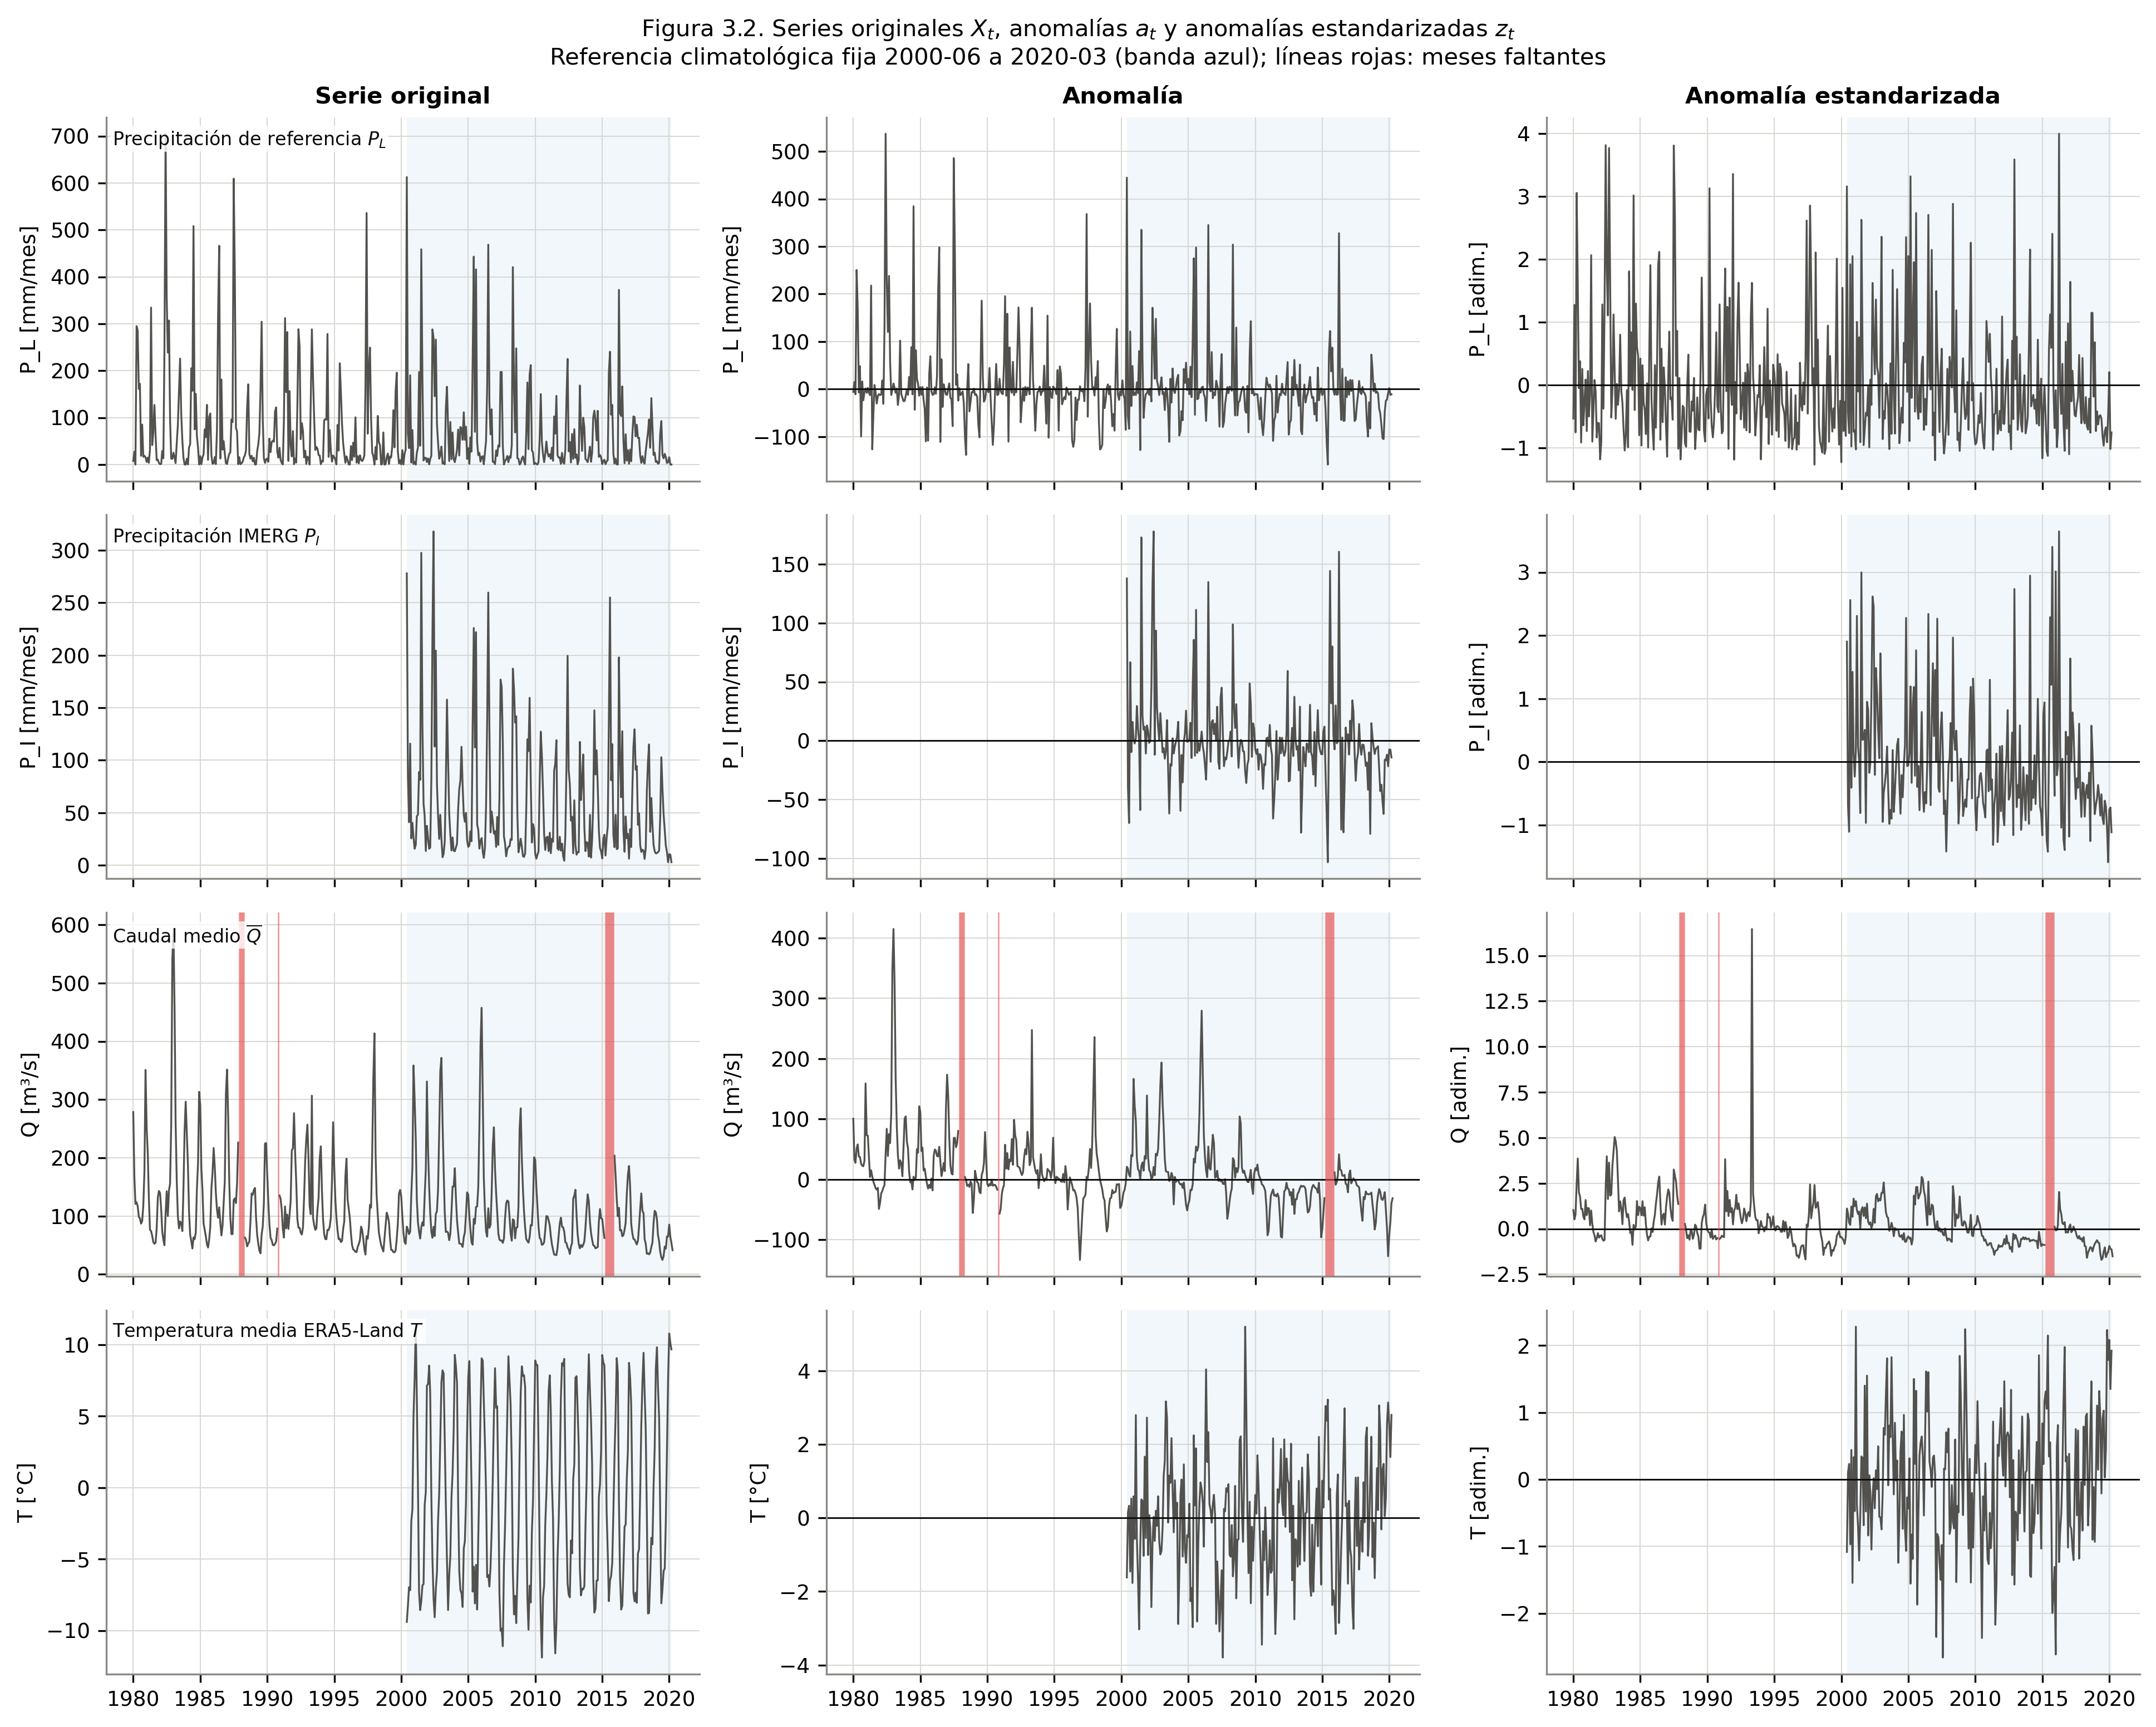
\includegraphics[width=\textwidth]{figura_3_2_representaciones.png}
\caption{Series originales $X_t$, anomalías $a_t$ y anomalías estandarizadas $z_t$ de $P_L$, $P_I$,
$\overline{Q}$ y $T$. Banda azul: referencia climatológica 2000-06 a 2020-03. Líneas rojas: meses faltantes
(no rellenados). Script \texttt{09\_p3\_2\_anomalias.py}.}
\label{fig:rep}
\end{figure}

\paragraph{Dos escalas (3.3).} Se evaluó (i) la secuencia cronológica de todos los meses y (ii) doce subseries
por mes calendario, en las tres representaciones y con el año decimal de las fechas reales como variable
temporal. Se comprobó numéricamente que, dentro de cada mes y con la misma muestra, la pendiente OLS de $a$
coincide con la de $X$ y la de $z$ es la de $X$ dividida por $s_j$ (diferencia máxima $1.4\times10^{-14}$,
\texttt{tabla\_3\_3\_verificacion\_invarianza.csv}). Por lo tanto, mes a mes, $a$ y $z$ no son evidencias
independientes de tendencia: solo cambian unidades. A escala global sí difieren, porque $z$ pondera igual los
meses secos y los húmedos (Figuras~\ref{fig:global} y \ref{fig:mensual}).

\begin{figure}[H]
\centering
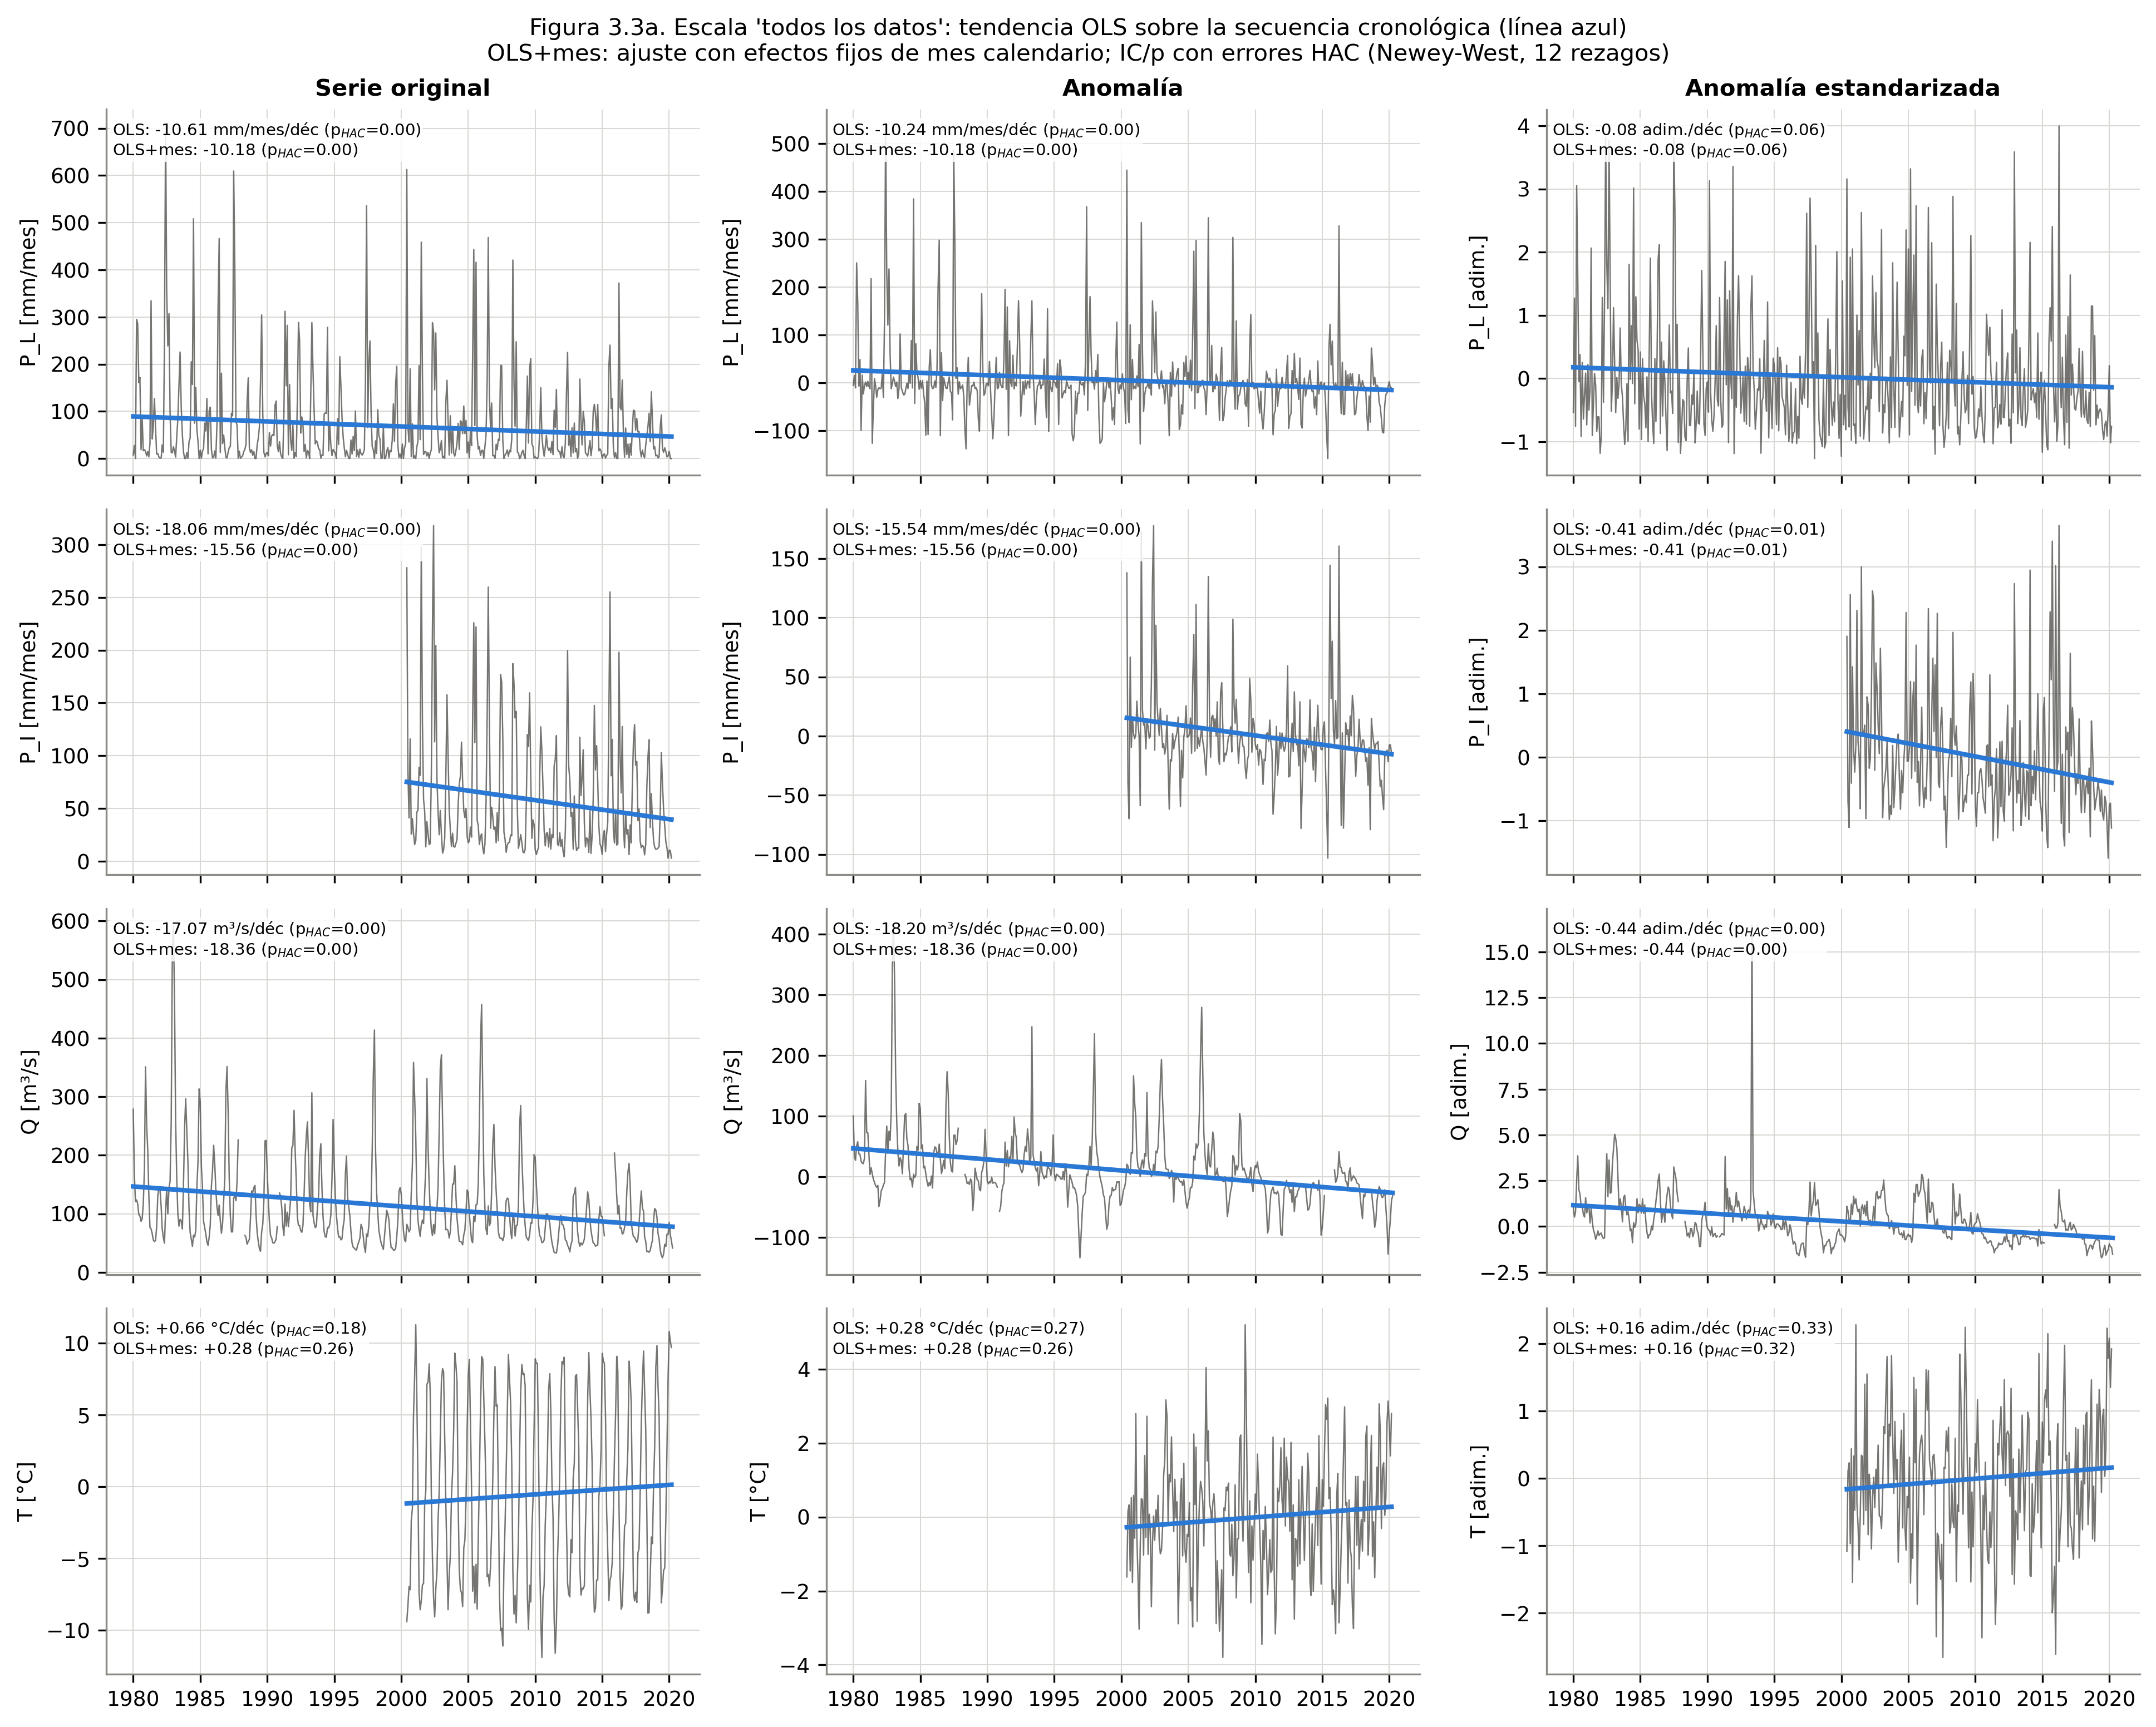
\includegraphics[width=\textwidth]{figura_3_3a_todos_los_datos.png}
\caption{Escala ``todos los datos'': tendencia OLS sobre la secuencia cronológica y, en el recuadro, el ajuste
con efectos fijos de mes calendario. Intervalos y valores $p$ con errores HAC (Newey--West, 12 rezagos).
Script \texttt{10\_p3\_3\_escalas\_temporales.py}.}
\label{fig:global}
\end{figure}

\begin{figure}[H]
\centering
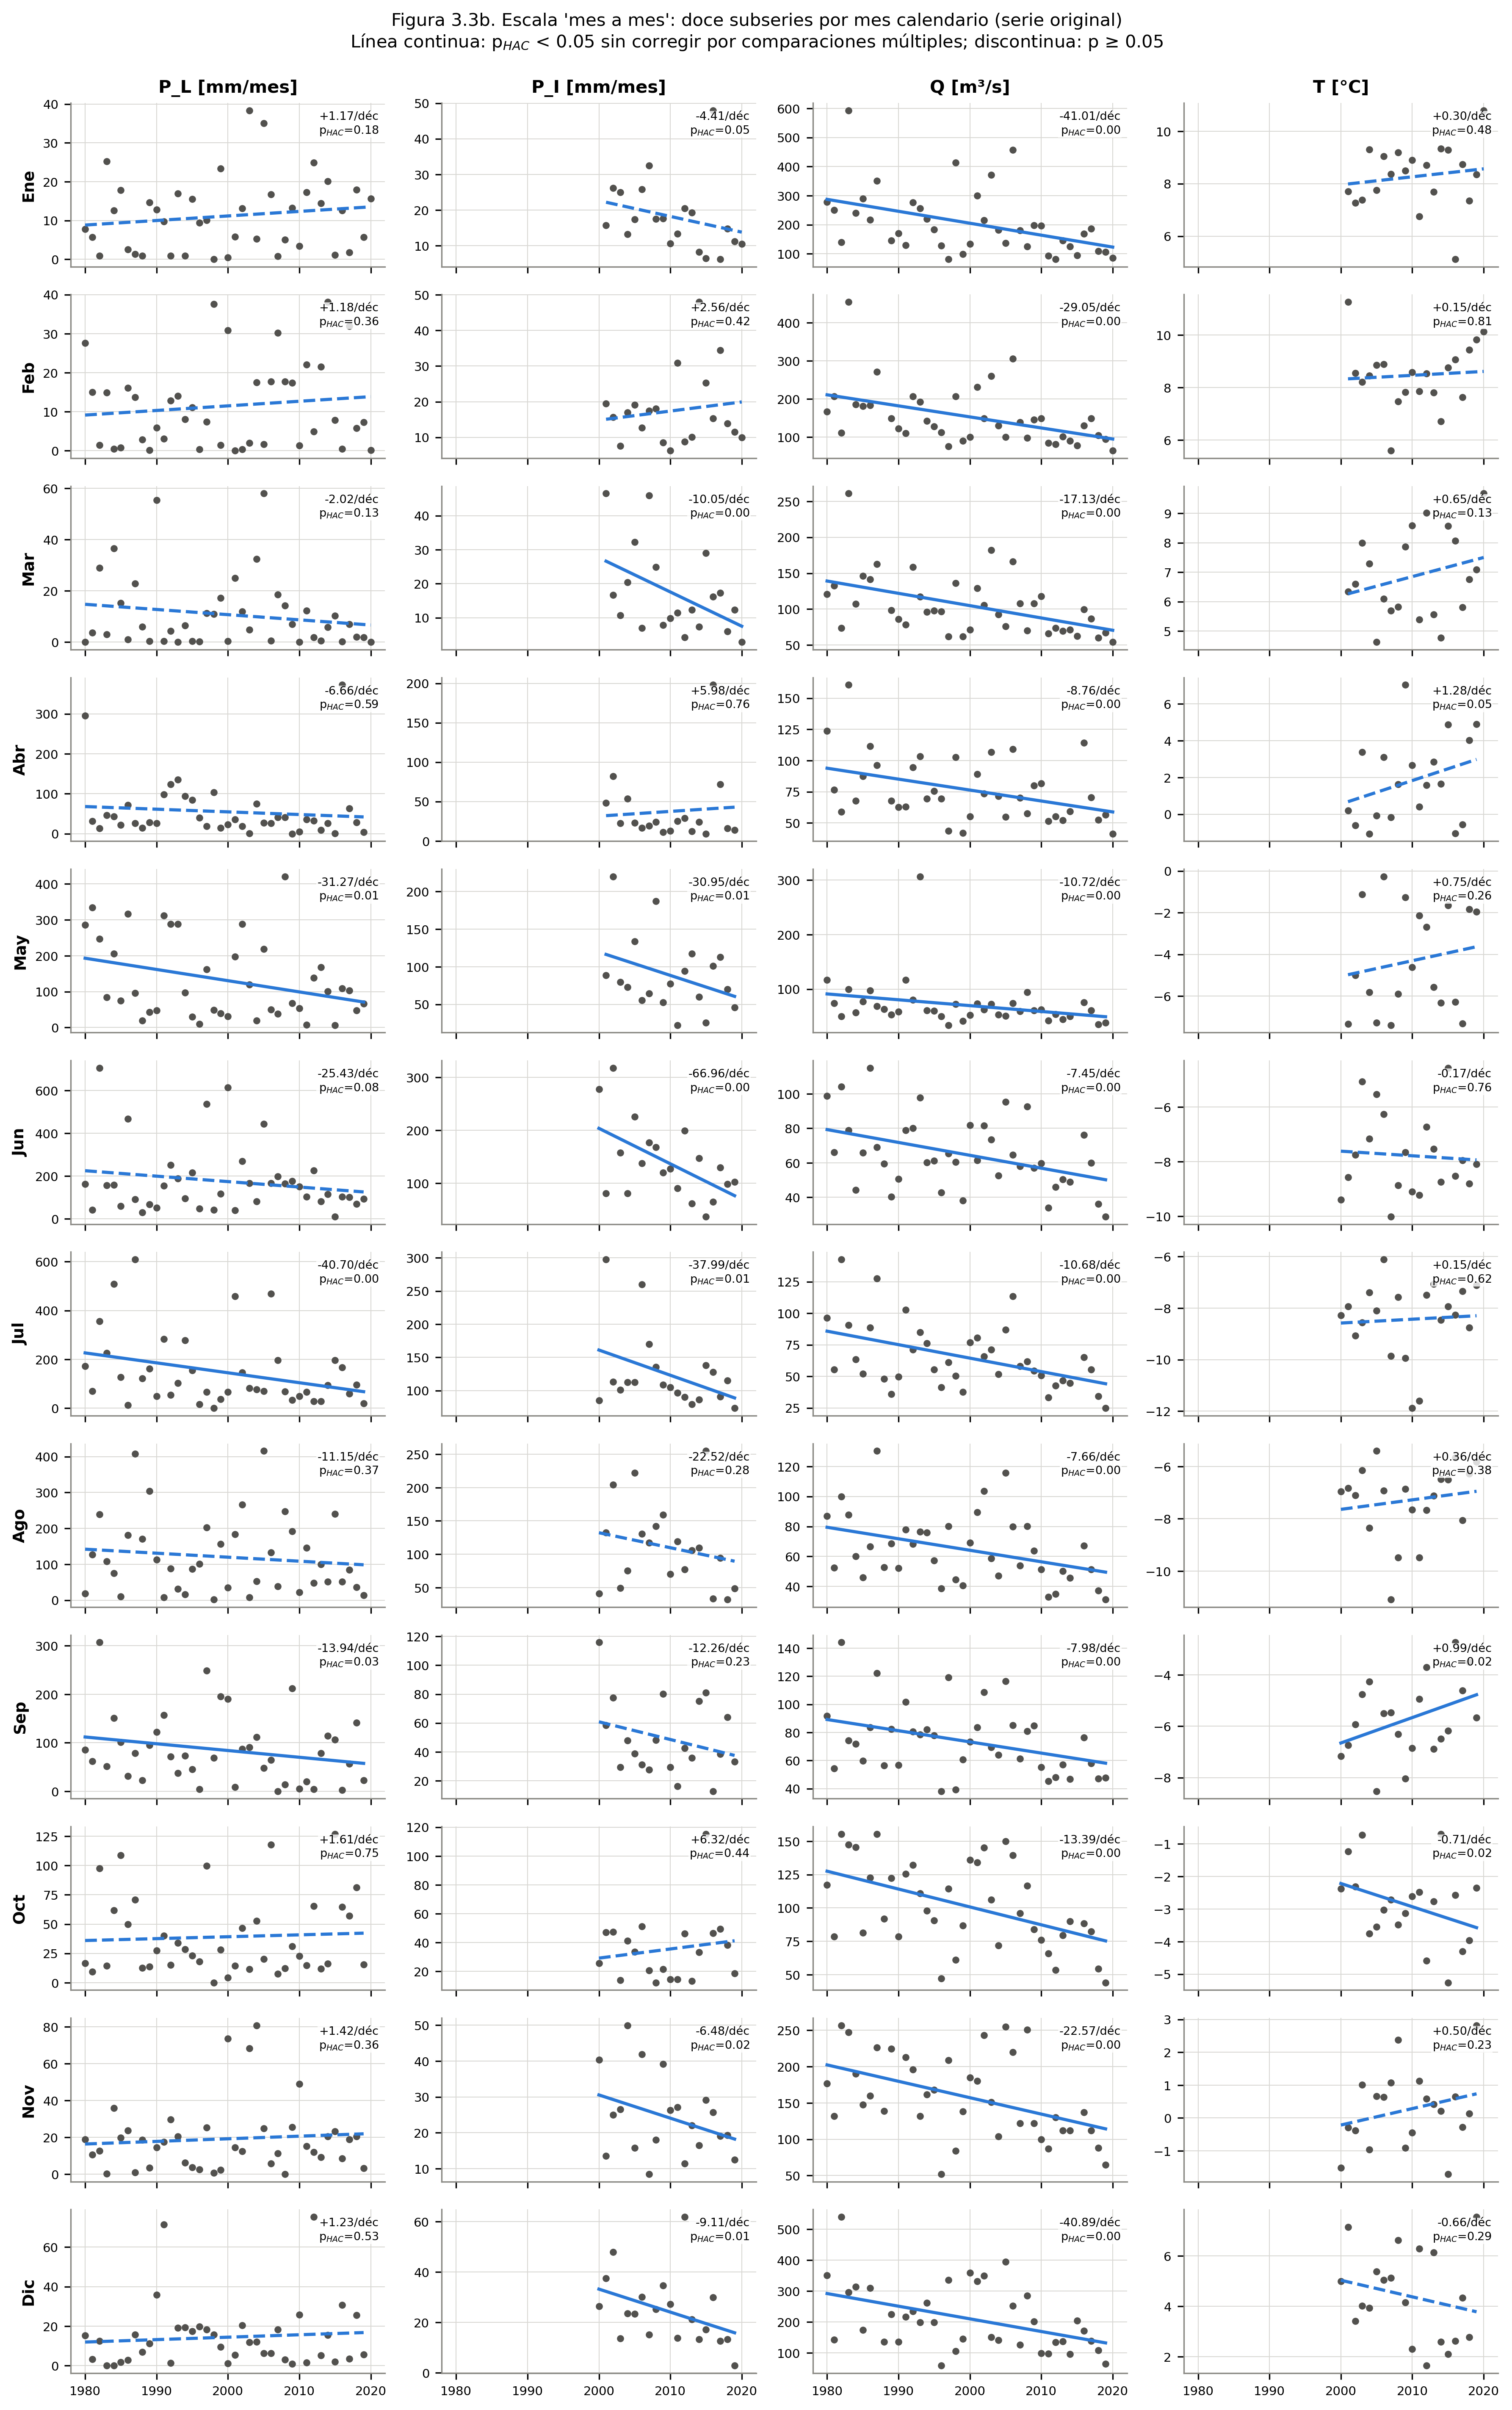
\includegraphics[height=0.82\textheight,keepaspectratio]{figura_3_3b_subseries_mensuales.png}
\caption{Escala ``mes a mes'': doce subseries por mes calendario (serie original) con su recta OLS. Línea
continua: $p_{\mathrm{HAC}}<0.05$ sin corregir por comparaciones múltiples.}
\label{fig:mensual}
\end{figure}

\paragraph{Métodos (3.4).} (1) OLS $X_t=\beta_0+\beta_1t+\varepsilon_t$ y su equivalente en $a$ y $z$; en la serie
original, además, un ajuste con efectos estacionales; inferencia con errores HAC \citep{NeweyWest1987} y
diagnóstico de residuos (Durbin--Watson, Ljung--Box, Breusch--Pagan). (2) Mann--Kendall \citep{Mann1945,Kendall1975}
con pendiente de Theil--Sen \citep{Sen1968}: Kendall estacional y Sen estacional para $X$ \citep{Hirsch1982},
con valor $p$ también por remuestreo de bloques de tres años completos \citep{Kundzewicz2004}; para $a$, $z$
y las doce subseries, la corrección de varianza por autocorrelación de Hamed y Rao \citep{HamedRao1998} (acotada para no
reducir nunca la varianza). (3) LOESS robusto \citep{Cleveland1979} con ventana de $\sim$10 años en la escala
global (banda del 95\,\% por bootstrap de bloques de 24 meses) y $\sim$15 años mes a mes; se usa como curva
exploratoria, sin inferencia. Nivel de significancia fijo $\alpha=0.05$ y control de falsos descubrimientos
\citep{BH1995,Wilks2016} con dos familias: 48 pruebas mensuales (12 meses $\times$ 4 variables) por método y
12 pruebas globales.

\begin{table}[H]
\centering\footnotesize
\caption{Comparación de métodos a escala global. Pendientes por década; en precipitación es el cambio del
\emph{acumulado mensual} (mm/mes por década), no del total anual. IC del 95\,\%. $q$: valor ajustado por FDR
(familia global de 12 pruebas). Fuente: \texttt{tabla\_3\_5\_comparacion\_metodos.csv} y \texttt{tabla\_3\_5\_fdr\_global.csv}.}
\label{tab:metodos}
\begin{tabular}{llrlrr}
\toprule
Variable (periodo, $n$) & Método & Pendiente & IC 95\,\% & $p$ & $q_{\mathrm{FDR}}$ \\
\midrule
$P_L$ (1980--2020, 483) & OLS sobre $a$ (HAC) & $-10.2$ & $[-17.3,\,-3.2]$ & 0.004 & 0.010 \\
 & Theil--Sen sobre $a$ (MK Hamed--Rao) & $-3.2$ & $[-6.8,\,-0.3]$ & 0.028 & 0.042 \\
 & Sen estacional sobre $X$ (bootstrap) & $-1.1$ & $[-2.9,\,0.1]$ & 0.080 & 0.107 \\
 & OLS sobre $z$ [z/déc] & $-0.08$ & $[-0.16,\,0.01]$ & 0.064 & -- \\
\midrule
$P_I$ (2000--2020, 238) & OLS sobre $a$ (HAC) & $-15.5$ & $[-26.0,\,-5.1]$ & 0.004 & 0.010 \\
 & Theil--Sen sobre $a$ (MK Hamed--Rao) & $-9.3$ & $[-15.9,\,-3.2]$ & 0.002 & 0.009 \\
 & Sen estacional sobre $X$ (bootstrap) & $-8.1$ & $[-12.6,\,-4.7]$ & 0.013 & 0.023 \\
\midrule
$\overline{Q}$ (1980--2020, 470) & OLS sobre $a$ (HAC) & $-18.2$ & $[-26.7,\,-9.7]$ & $<0.001$ & $<0.001$ \\
 & Theil--Sen sobre $a$ (MK Hamed--Rao) & $-14.9$ & $[-22.3,\,-7.8]$ & $<0.001$ & $<0.001$ \\
 & Sen estacional sobre $X$ (bootstrap) & $-12.4$ & $[-14.8,\,-9.8]$ & 0.005 & 0.010 \\
 & OLS sobre $z$ [z/déc] & $-0.44$ & $[-0.64,\,-0.25]$ & $<0.001$ & -- \\
\midrule
$T$ (2000--2020, 238) & OLS sobre $a$ (HAC) [$^\circ$C/déc] & $+0.28$ & $[-0.22,\,0.78]$ & 0.27 & 0.27 \\
 & Theil--Sen sobre $a$ (MK Hamed--Rao) & $+0.29$ & $[-0.15,\,0.72]$ & 0.19 & 0.21 \\
 & Sen estacional sobre $X$ (bootstrap) & $+0.31$ & $[-0.02,\,0.67]$ & 0.094 & 0.11 \\
\bottomrule
\end{tabular}
\end{table}

\begin{figure}[H]
\centering
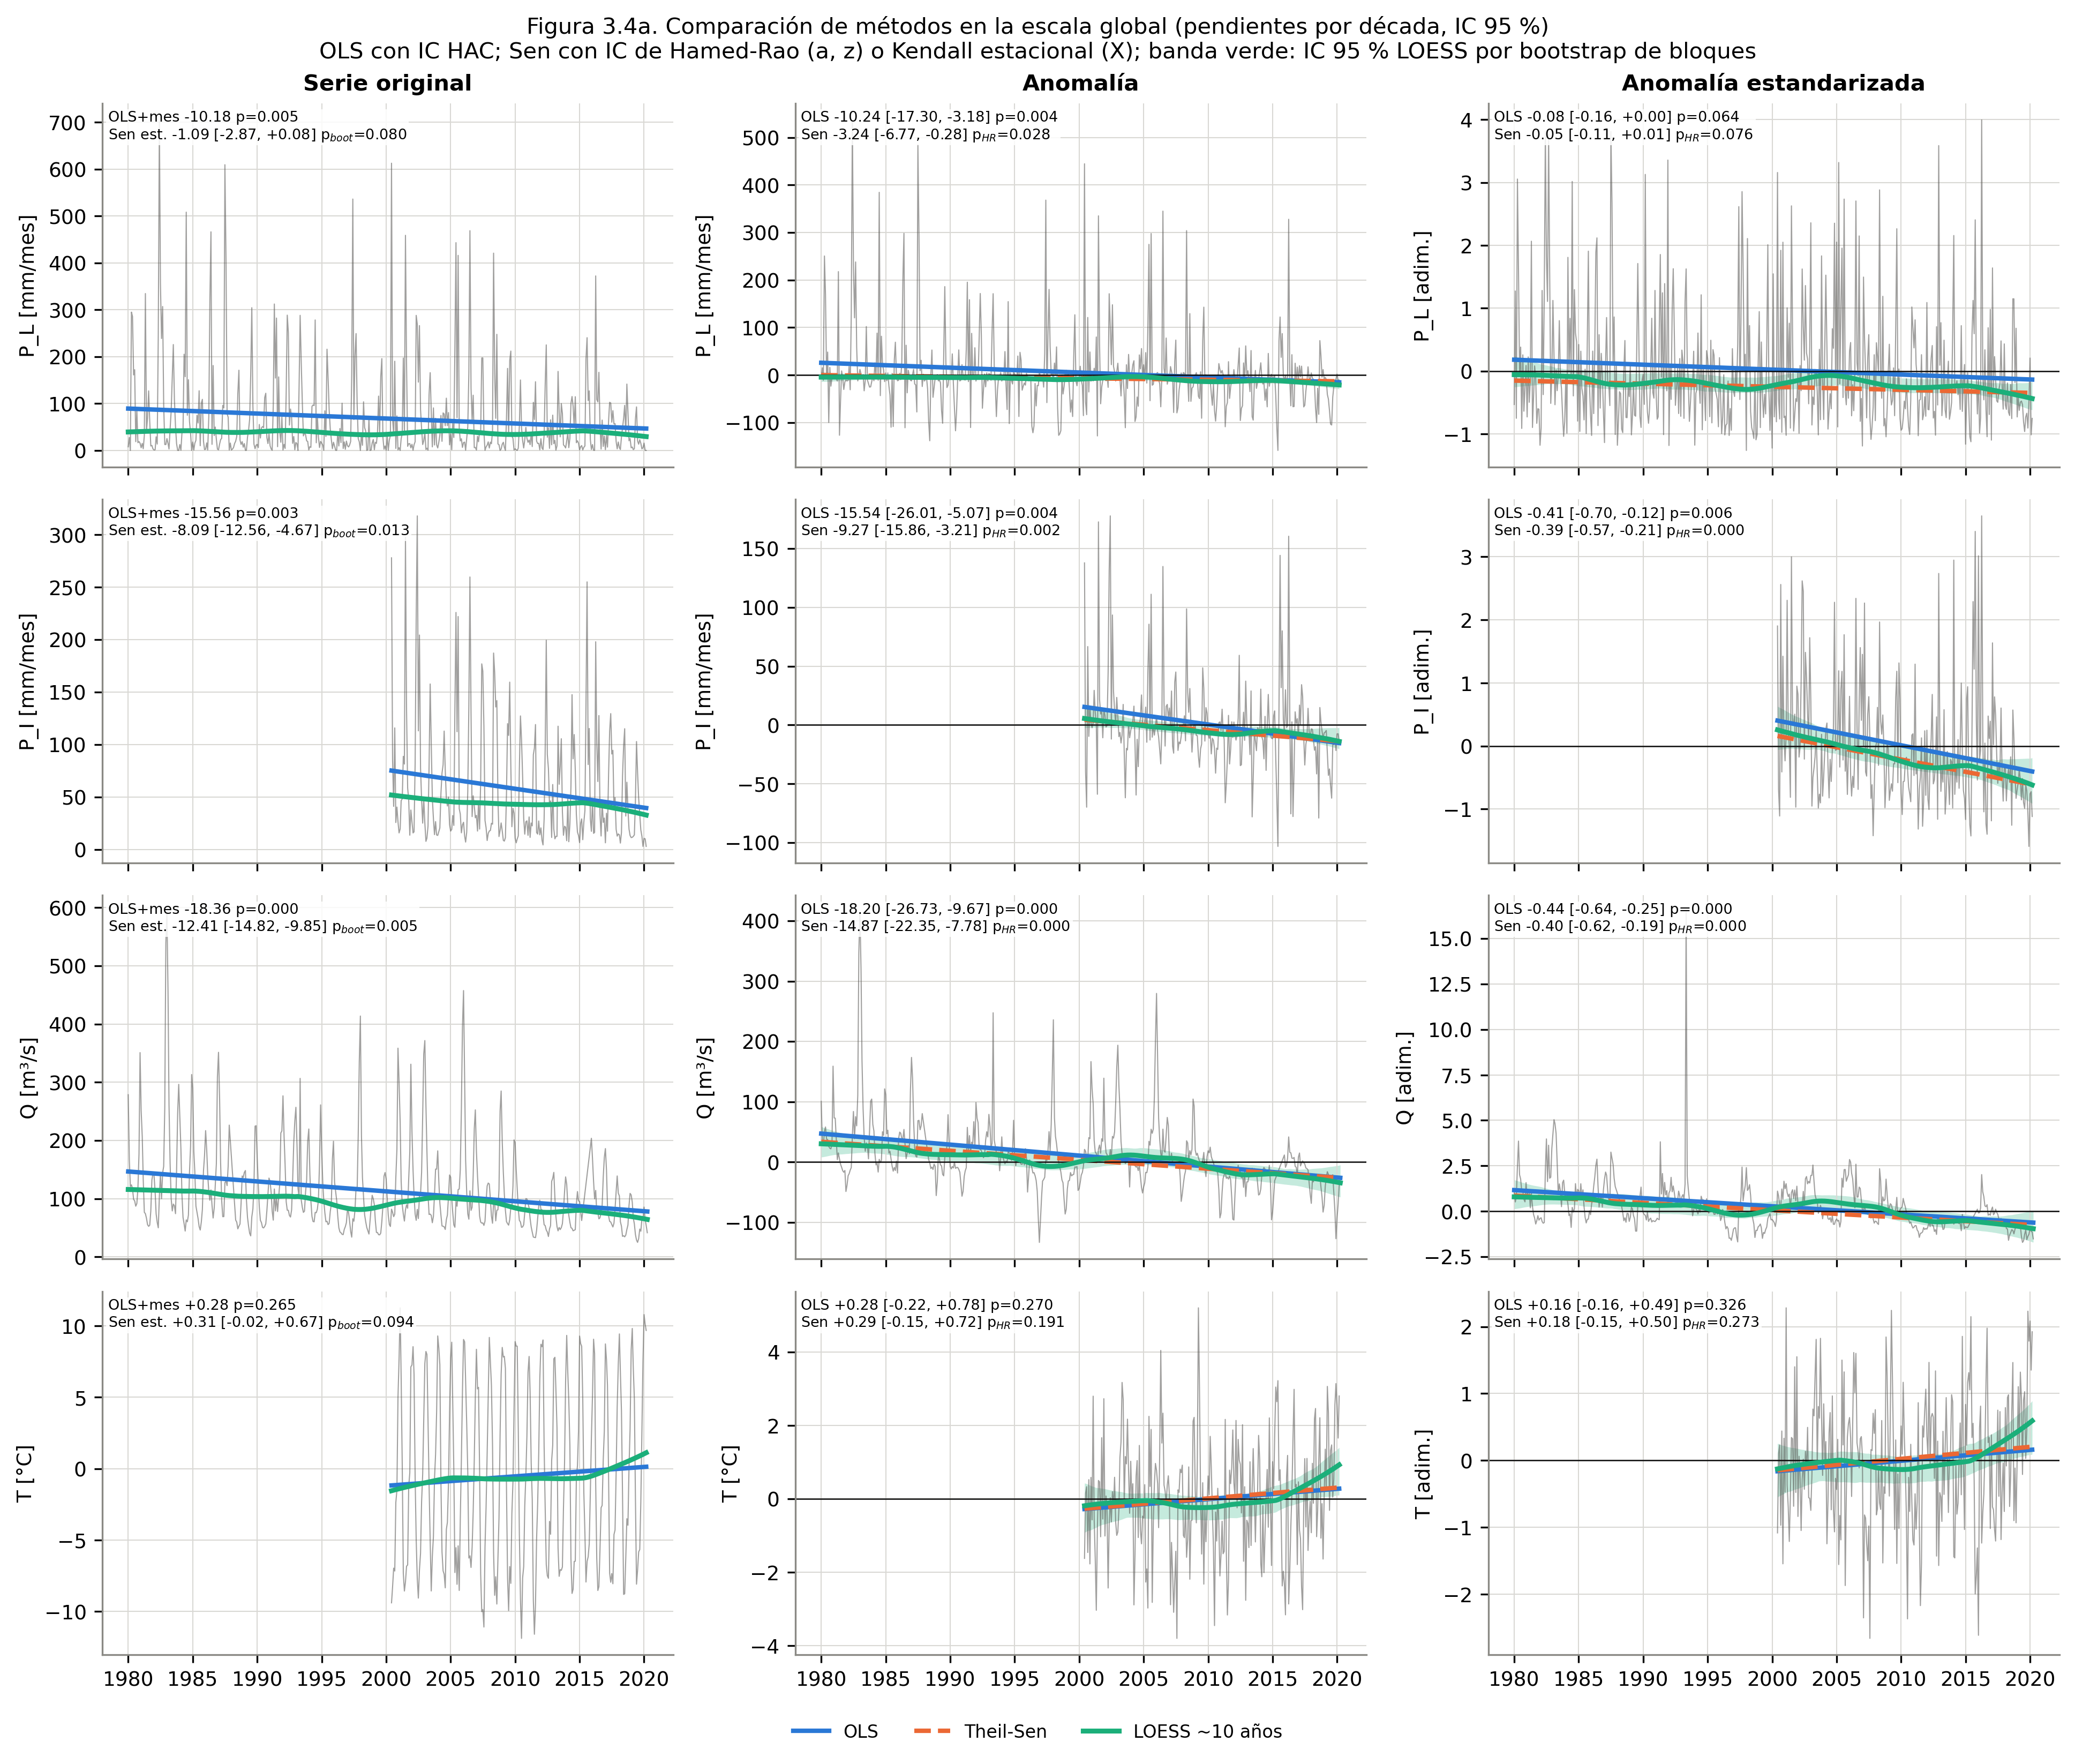
\includegraphics[width=\textwidth]{figura_3_4a_metodos_global.png}
\caption{Comparación de OLS (azul), Theil--Sen (naranja discontinua) y LOESS de $\sim$10 años (verde, con IC del
95\,\% por bootstrap de bloques) en las tres representaciones. Script \texttt{11\_p3\_4\_metodos\_tendencia.py}.}
\label{fig:metodos}
\end{figure}

Los residuos OLS presentan dependencia temporal clara (Figura~\ref{fig:resid}): en las anomalías de caudal la
autocorrelación de rezago 1 es 0.78 y Ljung--Box(12) rechaza independencia; en $P_L$ es 0.14 y Breusch--Pagan
indica heterocedasticidad ($p=0.02$). Por eso la inferencia se apoya en errores HAC y en las variantes de
Mann--Kendall corregidas, no en los errores estándar usuales. El factor de Hamed--Rao para $\overline{Q}$
(6.4 en $a$) confirma que la persistencia multiplica la varianza de $S$; aun así la tendencia sigue siendo
significativa.

\begin{figure}[H]
\centering
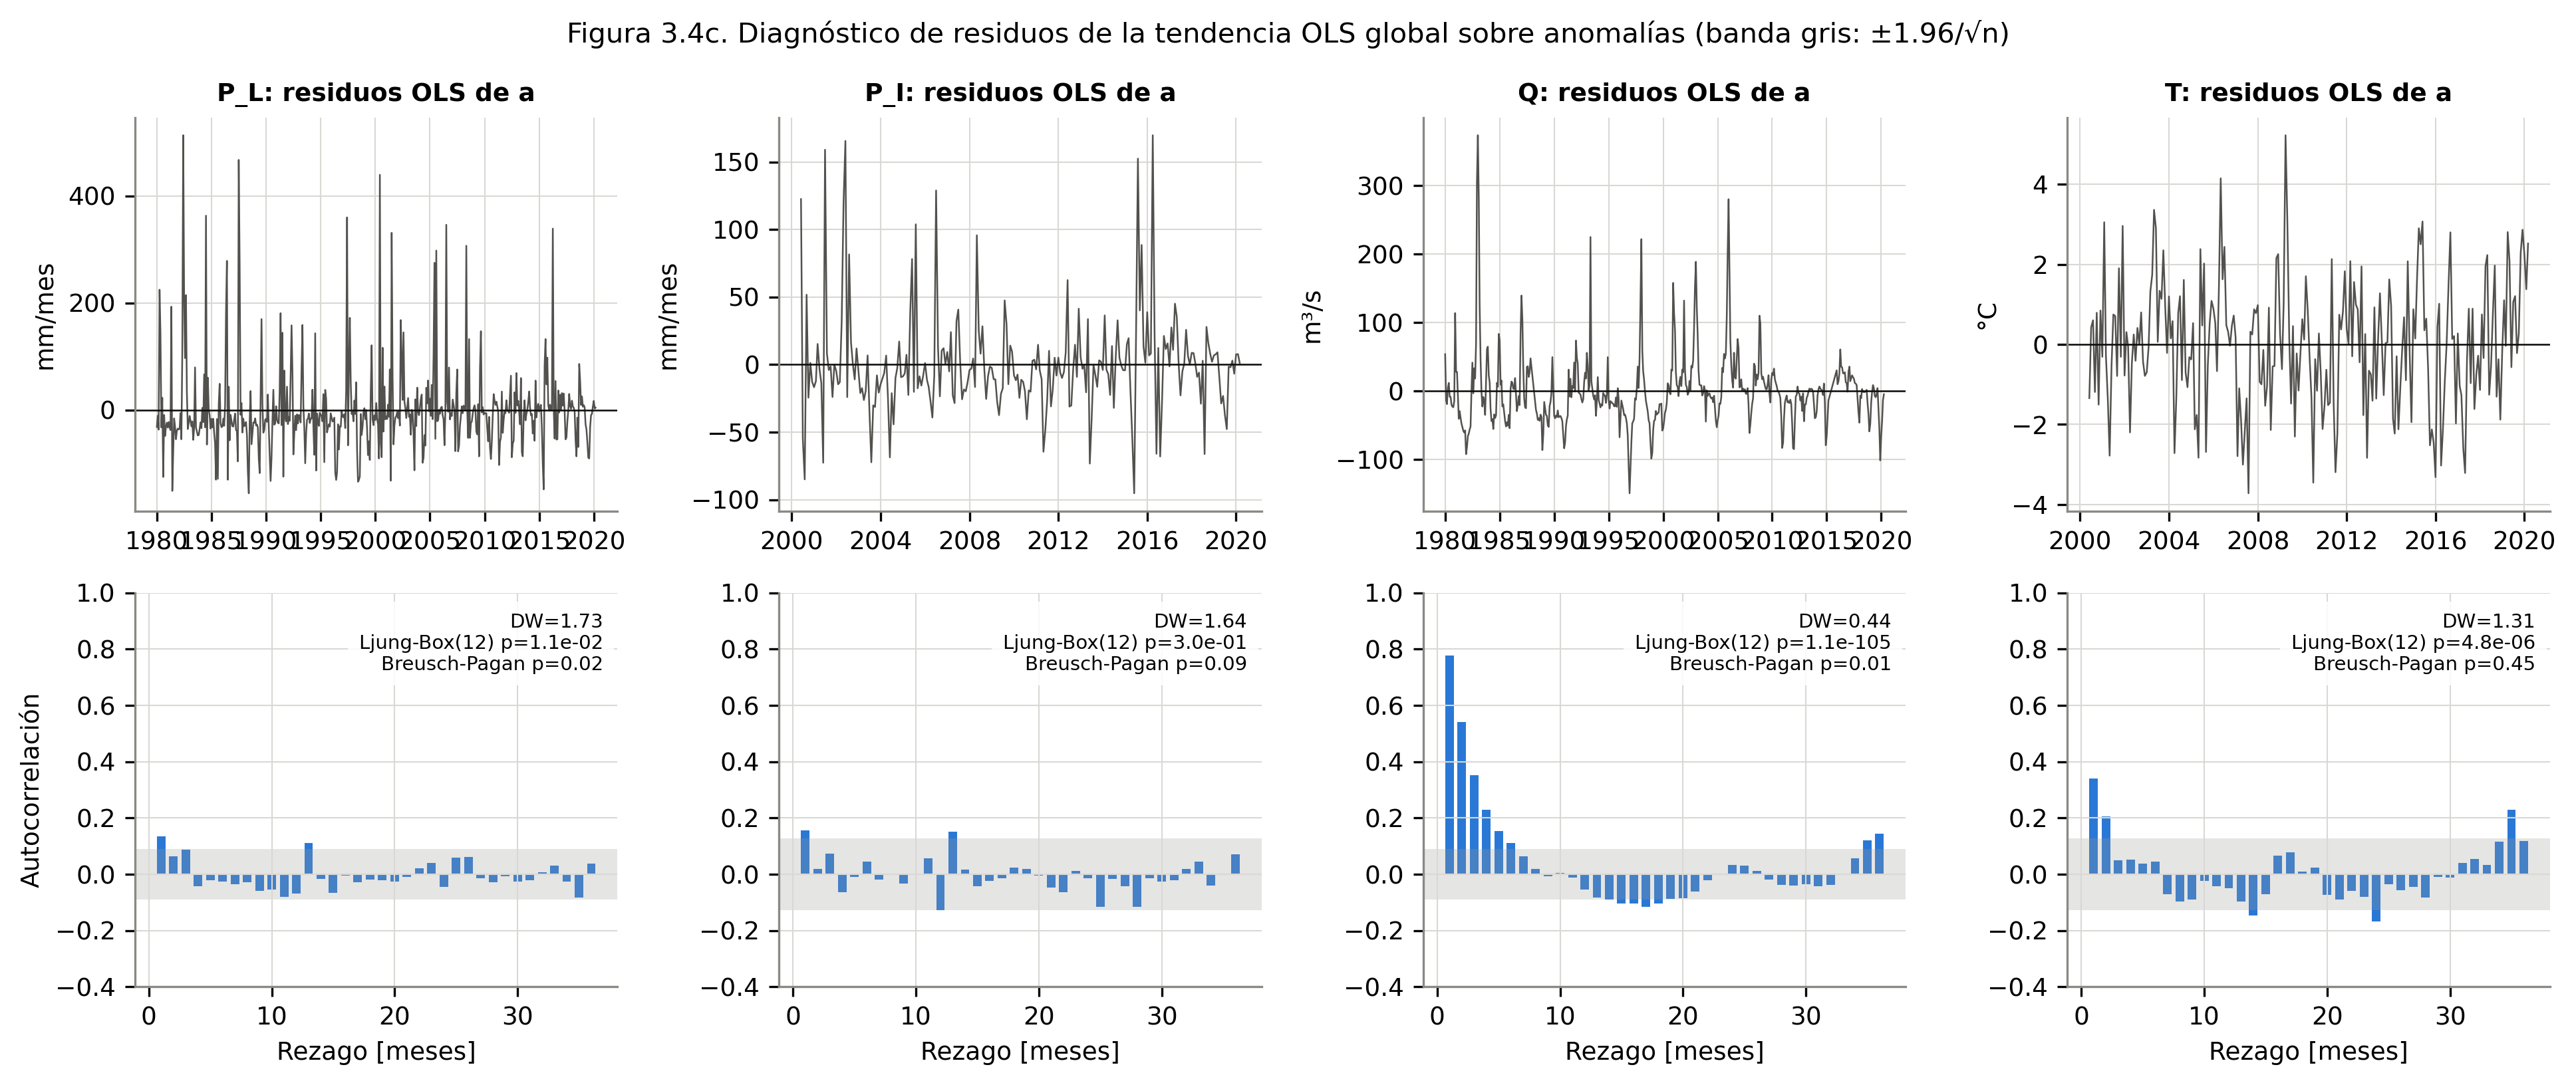
\includegraphics[width=\textwidth]{figura_3_4c_diagnostico_residuos.png}
\caption{Diagnóstico de residuos de la tendencia OLS global sobre anomalías: residuos en el tiempo y función
de autocorrelación (banda gris: $\pm1.96/\sqrt{n}$).}
\label{fig:resid}
\end{figure}

\begin{figure}[H]
\centering
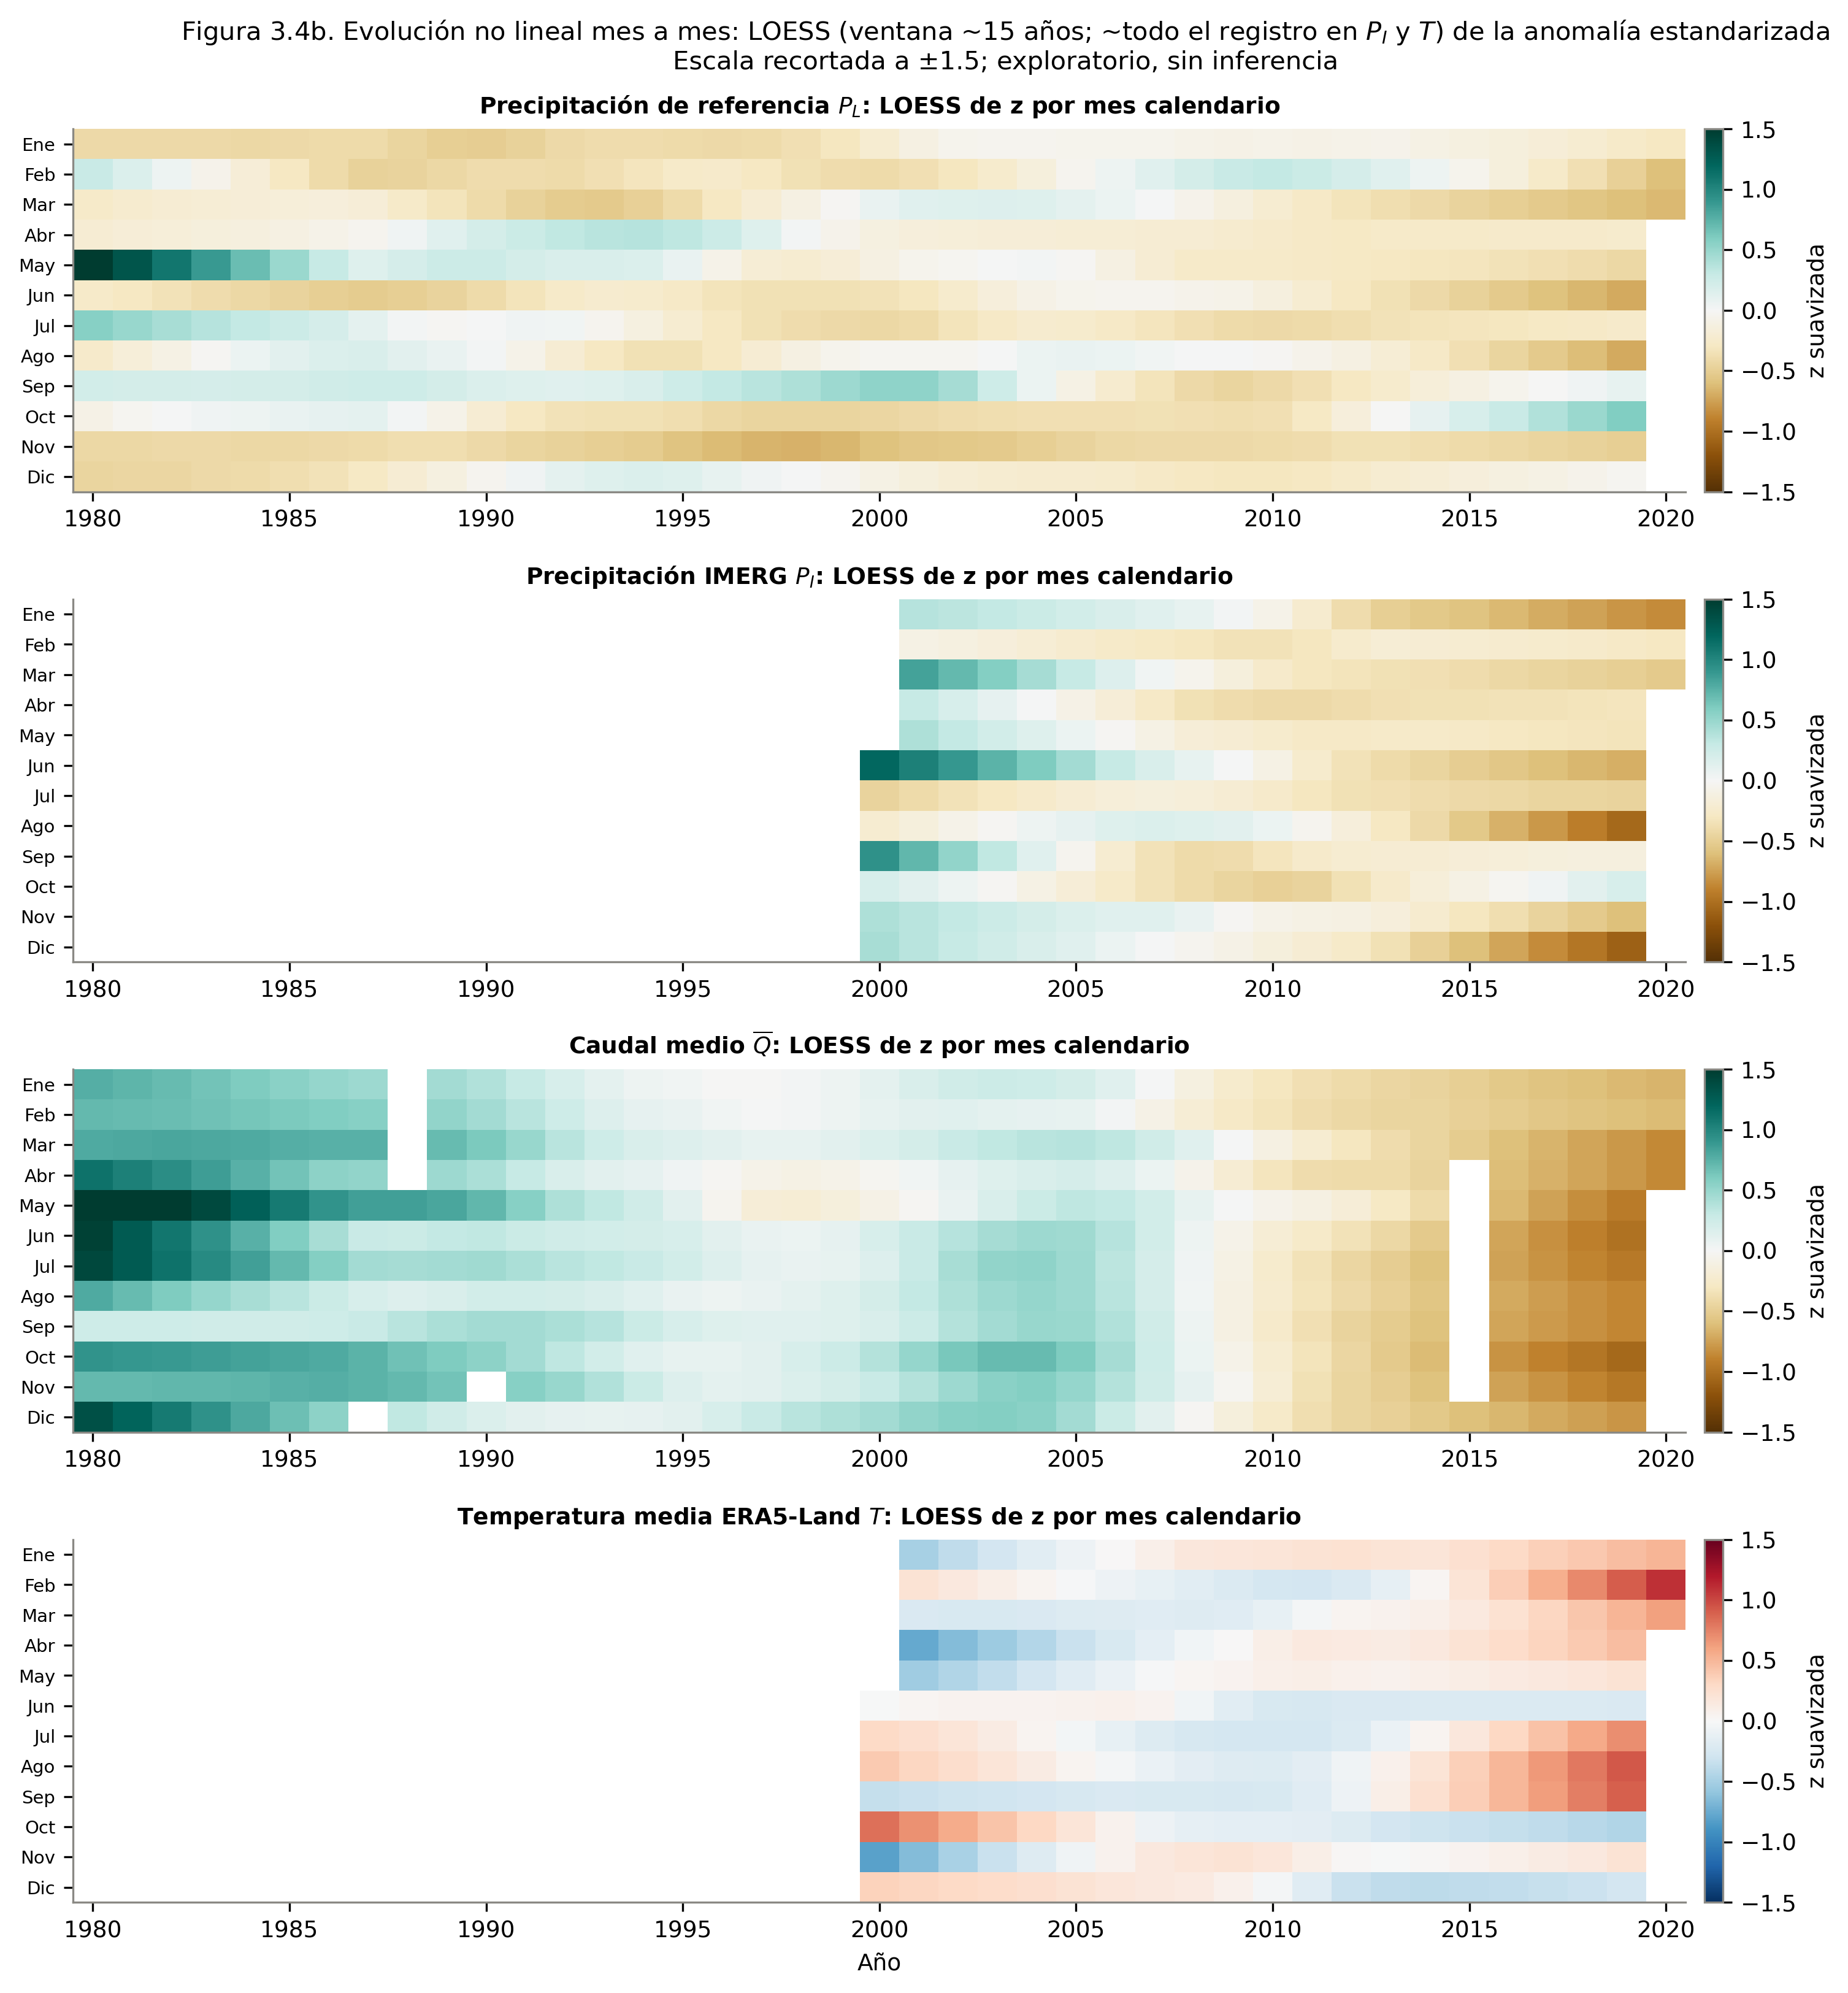
\includegraphics[width=\textwidth]{figura_3_4b_loess_mes_anio.png}
\caption{Evolución no lineal mes a mes: LOESS de la anomalía estandarizada de cada mes calendario (mapa
año--mes). Exploratorio; en $P_I$ y $T$ (20 años) la ventana abarca prácticamente todo el registro.}
\label{fig:loessmes}
\end{figure}

\paragraph{Incertidumbre y robustez (3.5).} La Figura~\ref{fig:pendmes} presenta las pendientes e intervalos
de los doce meses; la Figura~\ref{fig:inifin}, la sensibilidad a los años inicial y final; y la
Figura~\ref{fig:salto}, la comparación entre una tendencia gradual y un salto de nivel \citep{Pettitt1979}.
Las cifras se encuentran en \texttt{tabla\_3\_5\_sensibilidad.csv} y \texttt{tabla\_3\_5\_salto\_vs\_tendencia.csv}.

\begin{figure}[H]
\centering
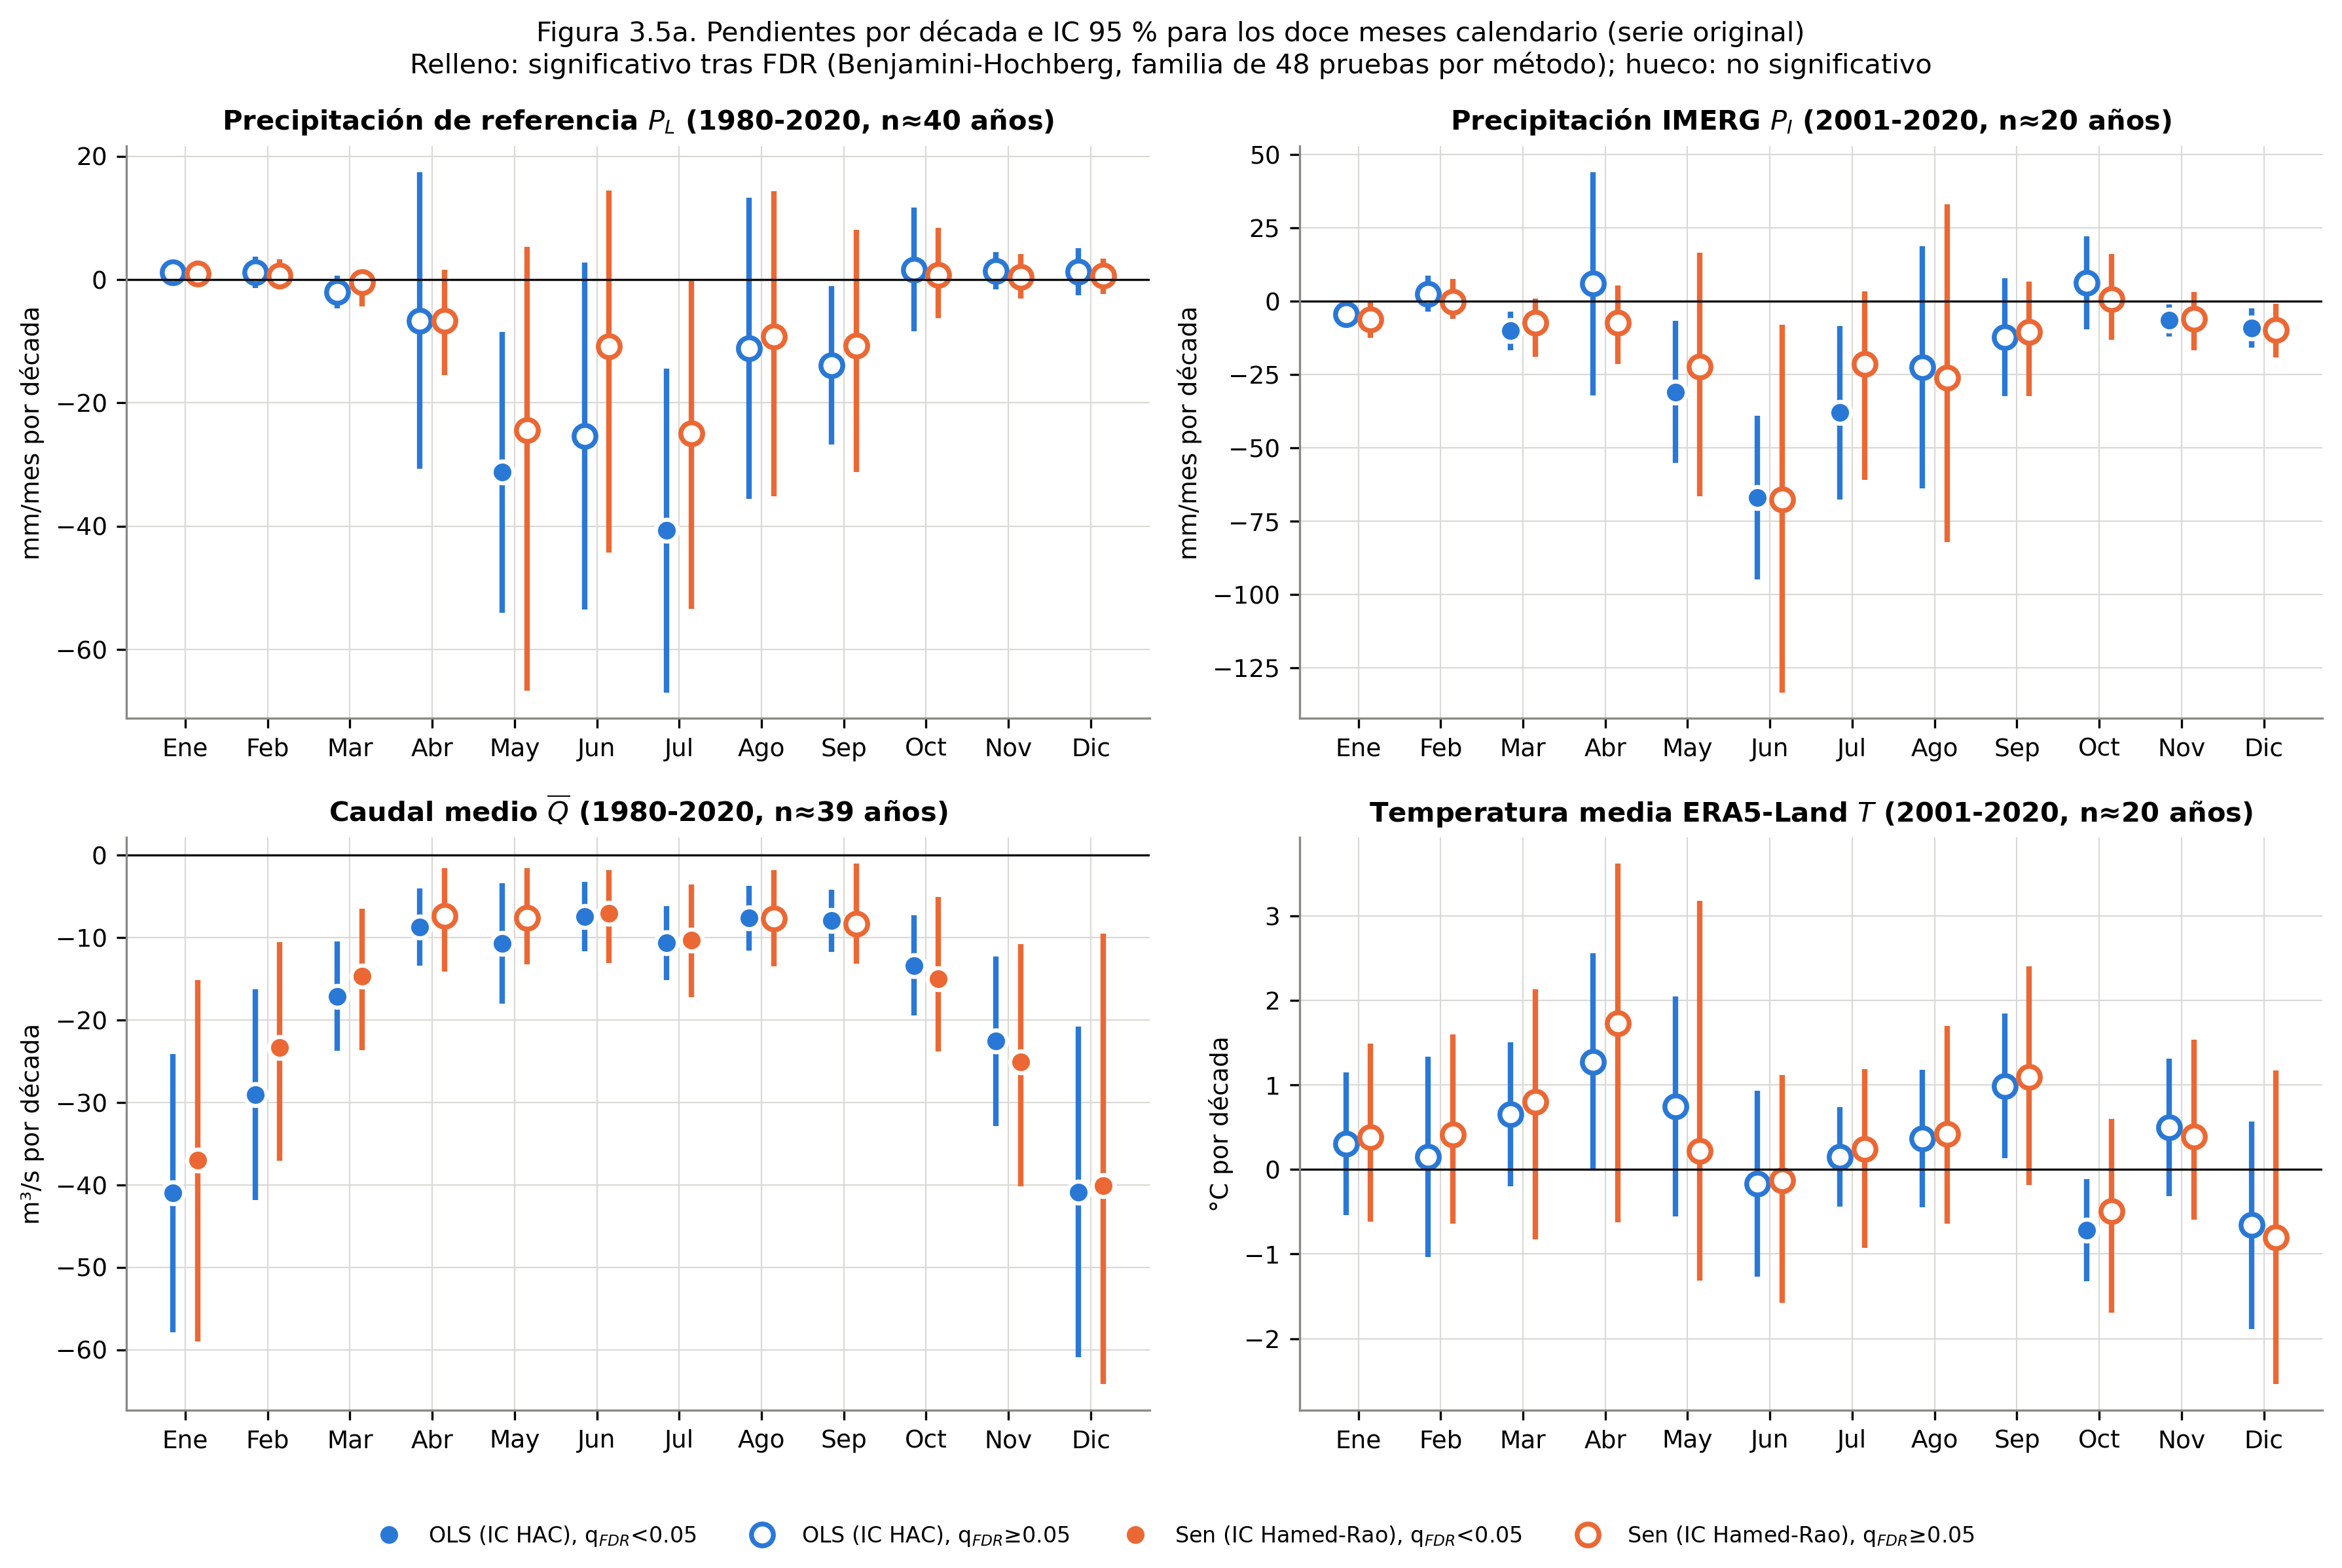
\includegraphics[width=\textwidth]{figura_3_5a_pendientes_mensuales_ic.png}
\caption{Pendientes por década e IC del 95\,\% para los doce meses (OLS con IC HAC y Sen con IC de Hamed--Rao).
Marcador relleno: significativo tras FDR en la familia de 48 pruebas de cada método. Script
\texttt{12\_p3\_5\_incertidumbre\_robustez.py}.}
\label{fig:pendmes}
\end{figure}

\begin{figure}[H]
\centering
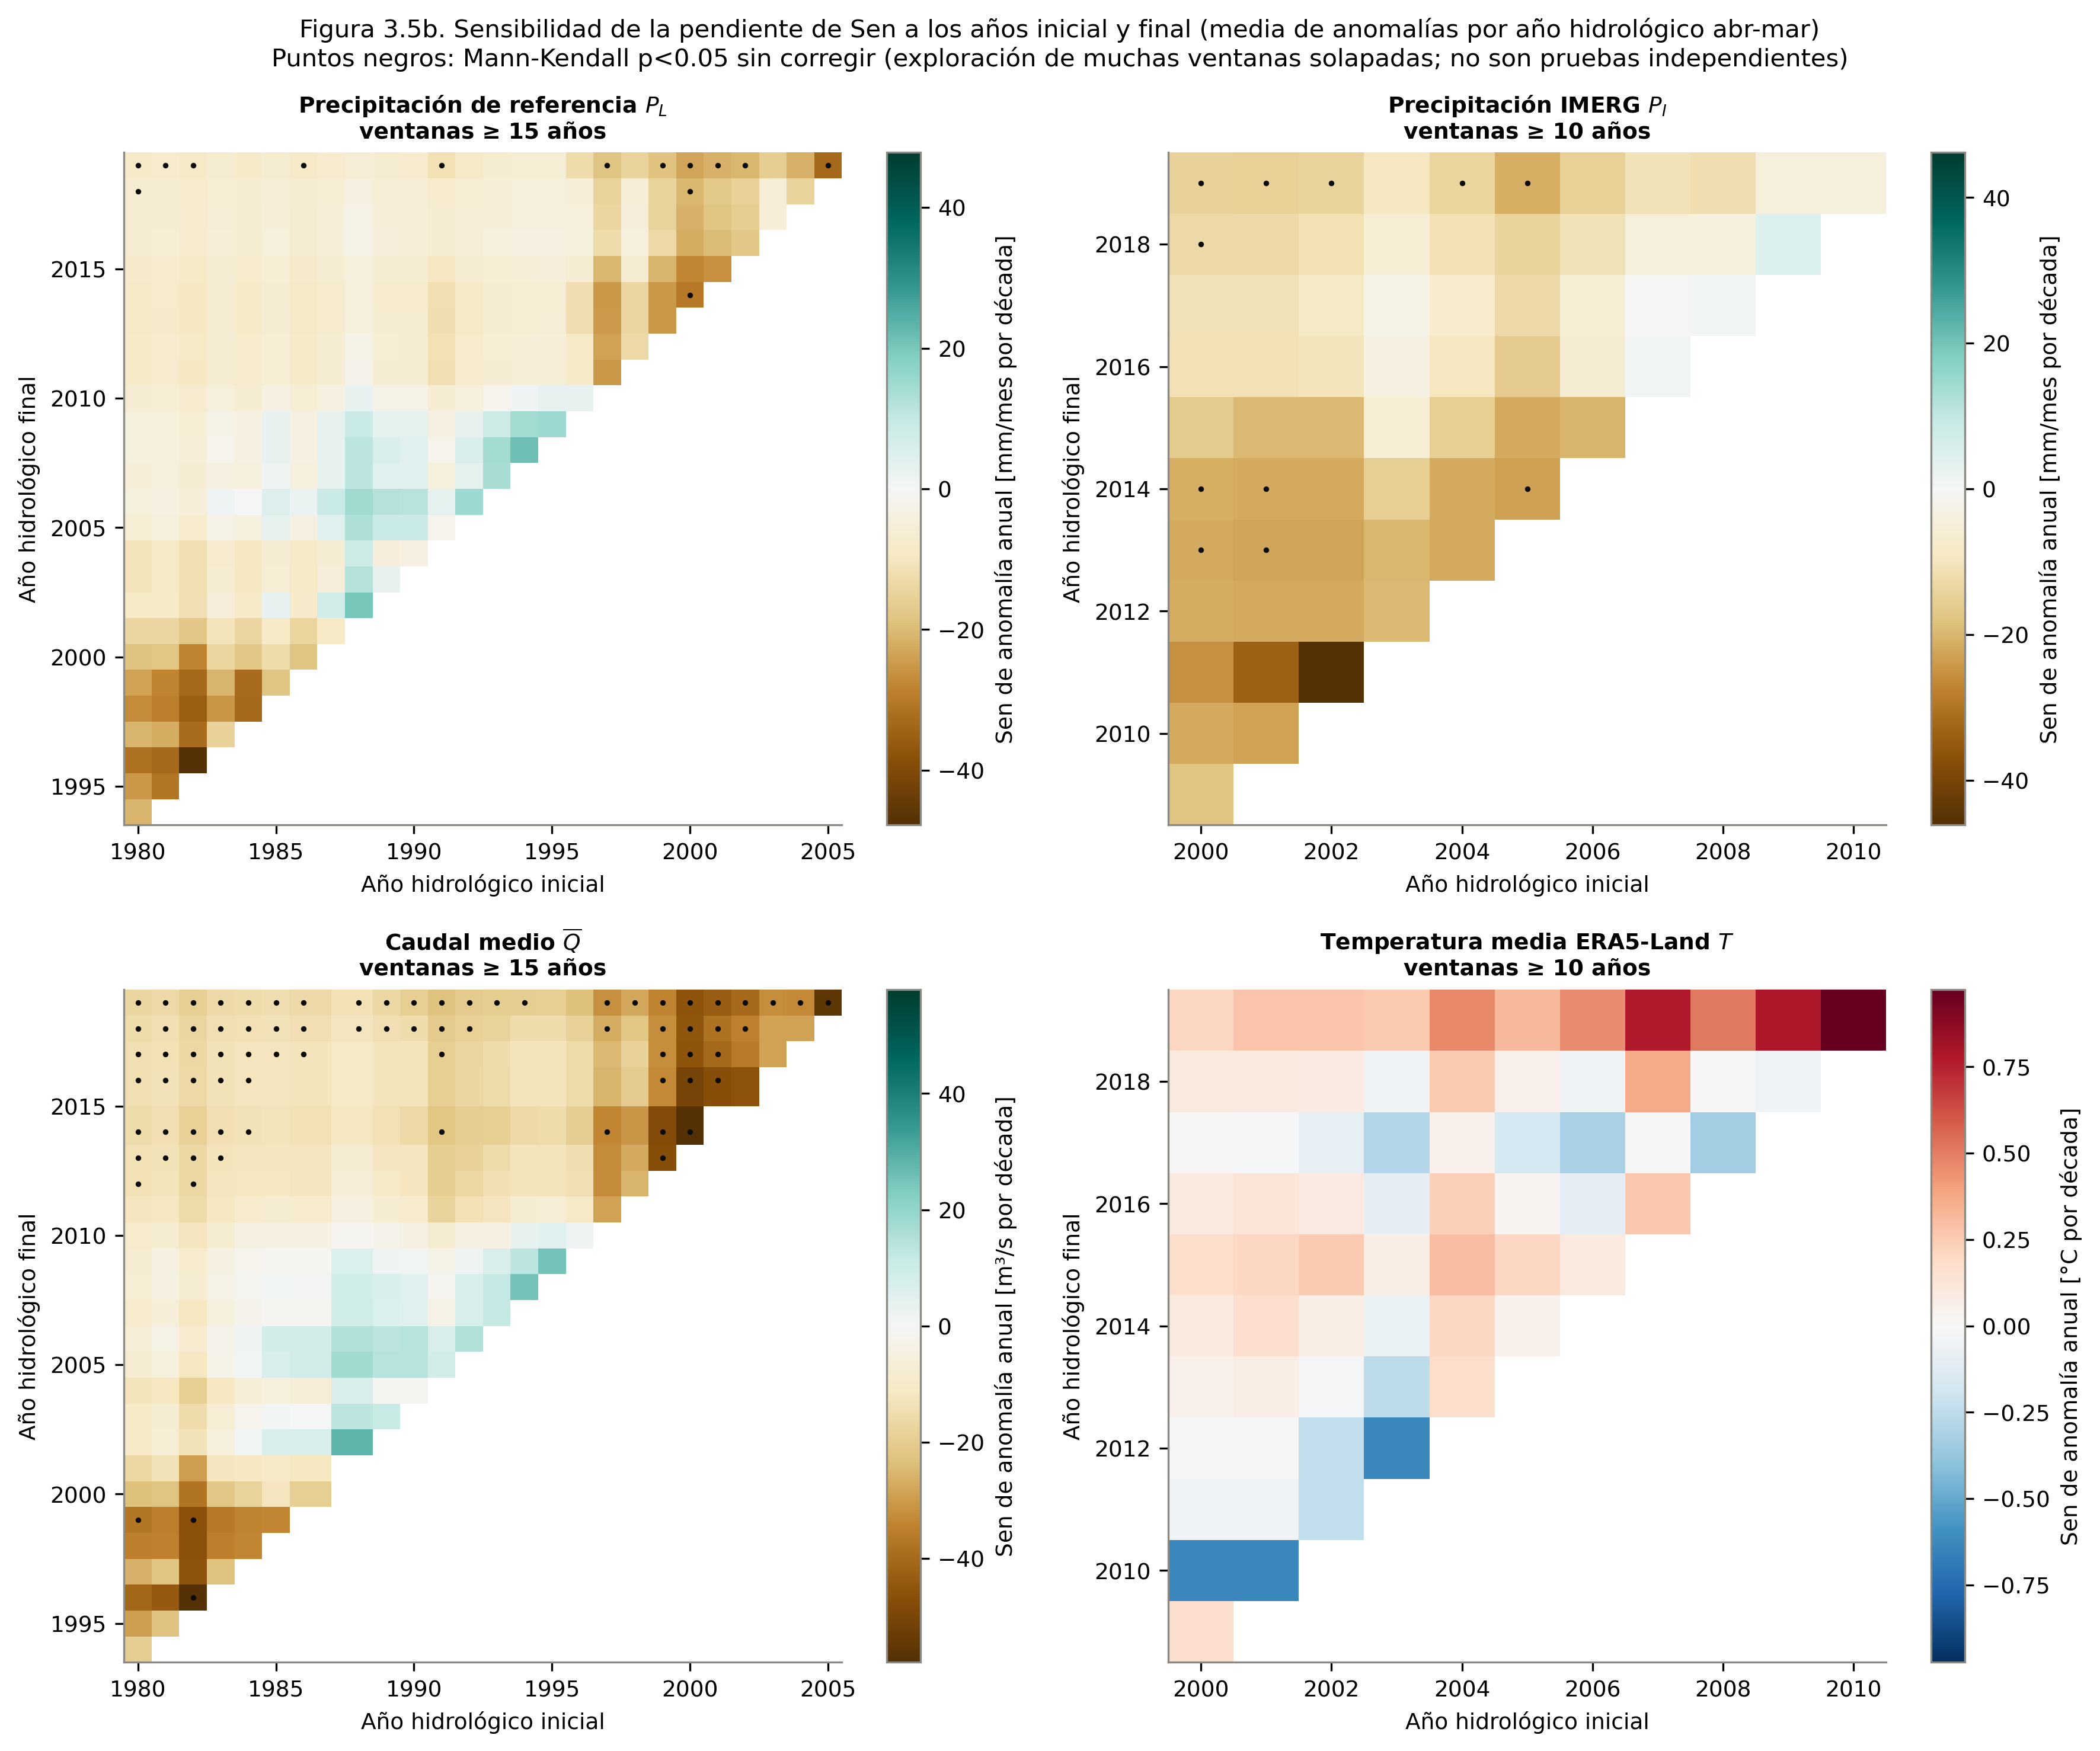
\includegraphics[width=\textwidth]{figura_3_5b_sensibilidad_inicio_fin.png}
\caption{Pendiente de Sen de la anomalía media por año hidrológico (abril--marzo) para todas las ventanas de
al menos 15 años ($P_L$, $\overline{Q}$) o 10 años ($P_I$, $T$). Puntos: Mann--Kendall $p<0.05$ sin corregir
(ventanas solapadas, no independientes).}
\label{fig:inifin}
\end{figure}

\begin{figure}[H]
\centering
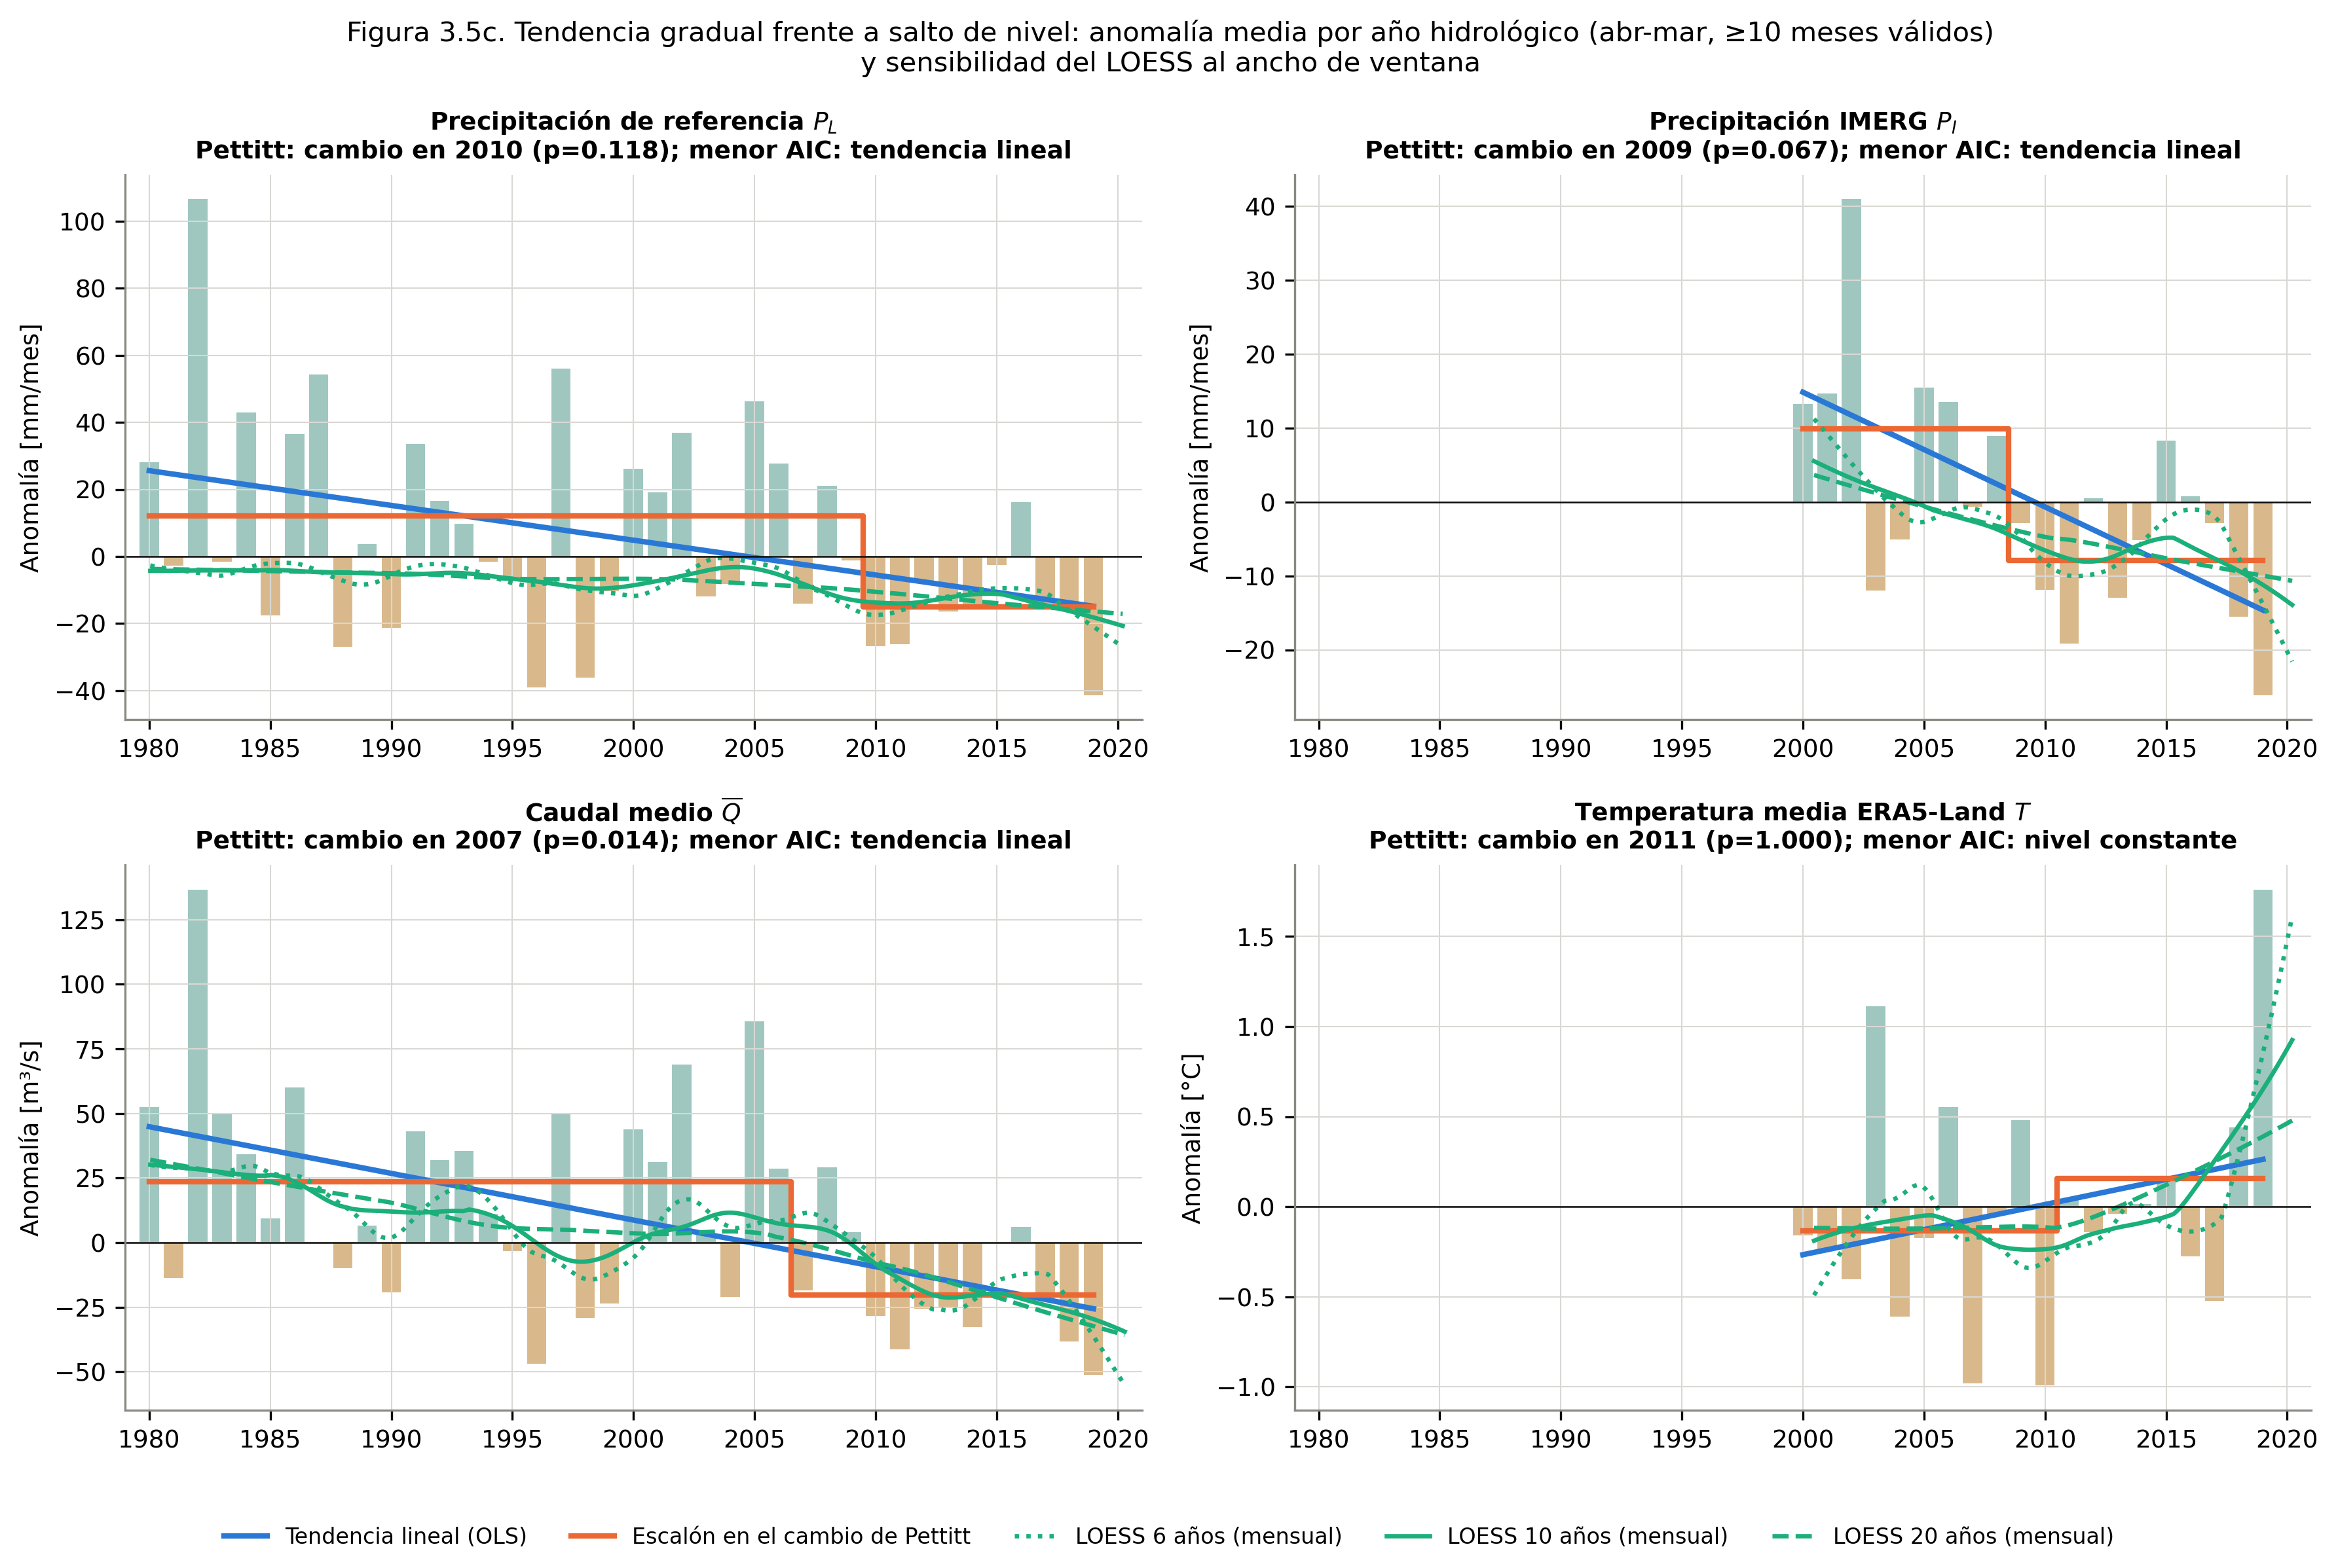
\includegraphics[width=\textwidth]{figura_3_5c_salto_vs_tendencia.png}
\caption{Anomalía media por año hidrológico con la tendencia lineal, el escalón en el punto de cambio de
Pettitt y LOESS con ventanas de 6, 10 y 20 años. El LOESS robusto queda por debajo de la media de los años
húmedos porque resta peso a las anomalías positivas extremas de una variable asimétrica.}
\label{fig:salto}
\end{figure}

\section{Síntesis de los resultados estadísticos}

\begin{enumerate}
\item \textbf{Caudal.} Disminuye en los doce meses y con todos los métodos y representaciones: entre $-12$ y
$-18$~m$^3$/s por década a escala global, y entre $-7$ y $-41$~m$^3$/s por década mes a mes (equivale a un
11--20\,\% de la media mensual por década). Los mayores descensos absolutos ocurren en diciembre--febrero,
los meses de deshielo (Figura~\ref{fig:pendmes}). Tras FDR, los 12 meses son significativos con OLS-HAC y
8 de 12 con Mann--Kendall corregido. Retirar los tres años hidrológicos más húmedos o el mayo de 1993 reduce
la magnitud (por ejemplo, de $-18.1$ a $-14.1$~m$^3$/s por década en la serie anual), pero no el signo ni la
significancia.
\item \textbf{Precipitación de referencia.} La disminución se concentra en el invierno (mayo, julio y
septiembre: $-31$, $-41$ y $-14$~mm/mes por década con OLS; 24--28\,\% de la media mensual por década en
mayo y julio), mientras que en verano las pendientes son nulas o ligeramente positivas. Tras FDR solo mayo y
julio siguen siendo significativos con OLS-HAC y ningún mes con Mann--Kendall. A escala global, OLS y Sen
sobre $a$ son significativos, pero el Sen estacional ($-1.1$, $p=0.08$) y $z$ ($p=0.06$) no lo son: estas dos
medidas dan el mismo peso a los meses secos de verano, que no cambian, y diluyen una señal que es invernal.
\item \textbf{IMERG.} En su registro de 20 años disminuye con todos los métodos ($-8$ a $-16$~mm/mes por década);
mes a mes, ninguna pendiente supera el FDR con Mann--Kendall.
\item \textbf{Temperatura (reanálisis).} Las pendientes son positivas ($+0.28$ a $+0.31$~$^\circ$C por década) pero
no significativas en 20 años. Hay un hallazgo metodológico: la OLS simple sobre $X$ da $+0.66$~$^\circ$C por
década, un sesgo de fase porque el registro empieza en invierno (junio de 2000) y termina en verano
(marzo de 2020); controlar la estacionalidad lo elimina ($+0.28$).
\item \textbf{Forma del cambio.} La caída no es lineal y homogénea. Hasta 2009 las pendientes de $P_L$
($-6.4$, $p=0.15$) y de $\overline{Q}$ ($-9.4$, $p=0.14$) no son significativas; el LOESS muestra fases
alternas (aumento 1998--2004, caída fuerte 2004--2013 y 2015--2020 en caudal), y Pettitt sitúa un cambio en
2007 para $\overline{Q}$ ($p=0.014$) y en 2010 para $P_L$ ($p=0.12$). Los modelos de tendencia lineal y de escalón
tienen AIC prácticamente iguales ($\Delta\mathrm{AIC}\approx0.2$): los datos no permiten distinguir una tendencia
gradual de un salto de nivel. Sí permiten afirmar que el signo negativo es mayoritario (86\,\% de las ventanas
de $\geq$15 años en $P_L$ y 85\,\% en $\overline{Q}$), aunque las ventanas que terminan entre 2002 y 2010 y
empiezan después de 1987 dan pendientes positivas.
\end{enumerate}

\section{¿A qué podrían deberse los cambios? (punto 3.6)}

\subsection{Contraste entre precipitación, caudal y temperatura}

\paragraph{¿Cambian en los mismos meses y periodos?} No en los mismos meses, pero sí en el mismo periodo y
de forma coherente con el régimen nivo-pluvial de la cuenca. La lluvia disminuye en los meses de acumulación
(mayo--septiembre), mientras que el caudal disminuye en todos los meses, con el máximo absoluto en
diciembre--febrero (Figuras~\ref{fig:pendmes} y \ref{fig:loessmes}). Esta transferencia estacional es la que
cabe esperar si el déficit de nieve invernal se traduce en menor deshielo en primavera y verano: en esta cuenca
la temperatura media es inferior a 0~$^\circ$C de mayo a octubre y el 70.9\,\% de la precipitación cae como nieve
según CAMELS-CL \citep{AlvarezGarreton2018}, y los roles A y B encontraron un desfase de unos 6--7 meses entre
el máximo de lluvia y el de caudal. La literatura regional muestra que la acumulación nival andina entre
30 y 37$^\circ$S controla el caudal de la temporada cálida \citep{Masiokas2006}. En el tiempo, $P_L$ y $\overline{Q}$
coinciden en el punto de cambio (2007--2010) y en las fases del LOESS, lo que sitúa el cambio principal en el
inicio de la megasequía de Chile central \citep{Garreaud2017,Garreaud2020}.

\paragraph{¿Responde el caudal de manera consistente con la precipitación?} En magnitud, sí. Por año
hidrológico completo, la lámina de precipitación media bajó de 915~mm (1980--2009, 27 años completos) a 557~mm
(2010--2019, 9 años), un $-39$\,\%, y la escorrentía bajó de 822 a 475~mm, un $-42$\,\%. La elasticidad aparente
es $\approx1.1$, y el coeficiente $R/P$ pasa de 0.95 a 0.90 sin tendencia significativa (Sen $-0.015$ por década,
$p=0.54$). Una regresión anual $R=-14.2+0.71P_t+0.20P_{t-1}$ ($R^2=0.92$) deja un residuo medio de
$+8$~mm/año antes de 2010 y de $-23$~mm/año después: tras descontar la lluvia del año y la del anterior queda
un déficit adicional pequeño. Es compatible con el agotamiento progresivo de almacenamientos (nieve
remanente, agua subterránea) descrito para cuencas chilenas de memoria larga durante sequías plurianuales
\citep{AlvarezGarreton2021}, aunque con solo nueve años posteriores a 2010 no es una prueba. El coeficiente
$R/P\approx0.9$ es muy alto para una cuenca semiárida; indica que $P_L$ podría subestimar la precipitación de
alta montaña o que hay aportes glaciares no despreciables \citep{Ayala2020}. Por eso estas cifras se leen como
consistencia relativa y no como un balance hídrico cerrado.

\paragraph{¿Podrían intervenir evapotranspiración, almacenamiento, nieve o deshielo?} La temperatura de
ERA5-Land no muestra una tendencia significativa en 2000--2020, pero el LOESS indica un calentamiento
concentrado después de 2009 ($+1.2$~$^\circ$C en la curva de anomalías hasta 2020) y años muy cálidos y secos al
final del registro (anomalías de $+1.7$ a $+3.1$~$^\circ$C entre noviembre de 2019 y marzo de 2020, junto con el año
más seco de $P_L$). Un calentamiento de esa magnitud elevaría la línea de nieves, adelantaría el deshielo y
aumentaría la sublimación y la evapotranspiración, mecanismos que podrían explicar el déficit residual de
caudal. Sin embargo, la serie térmica es corta, no significativa y procede de un reanálisis; la magnitud
($\sim$0.3~$^\circ$C por década) es comparable al calentamiento andino documentado para 1979--2006
\citep{Falvey2009}. La hipótesis térmica queda abierta: hacen falta temperatura de estaciones de altura,
equivalente en agua de nieve y caudales diarios para fechar el deshielo.

\paragraph{Rezagos y diferencias entre IMERG y la referencia.} Con la persistencia mensual del caudal
(autocorrelación de 0.78 en las anomalías), un déficit de lluvia afecta varios meses de caudal, lo que explica
que la tendencia del caudal tenga mayor evidencia estadística que la de la lluvia (Tabla~\ref{tab:metodos}).
En el periodo común, $P_L$ cae $-24.3$~mm/mes por década y $P_I$ $-15.5$ (anomalía anual), y la diferencia
$P_I-P_L$ por año hidrológico aumenta $+106$~mm/año por década ($p=0.06$): ambos productos coinciden en el signo,
pero no en la magnitud. El cociente anual $P_I/P_L$ varía entre 0.67 y 1.44 sin un patrón estable. Se discute
como posible inhomogeneidad observacional en la Sección~\ref{sec:obs}.

\subsection{Contexto de la cuenca}

Los cambios detectados deben contrastarse con intervenciones documentadas. Aguas arriba de El Manzano existe
el embalse El Yeso, que regula el río Yeso para el abastecimiento de agua potable de Santiago y opera desde la
década de 1960 \citep{AlvarezGarreton2018}. % VERIFICAR: capacidad, fecha de puesta en marcha y reglas de operación con DGA/Aguas Andinas; revisar atributos big_dam e interv_degree de CAMELS-CL para 5710001.
Como antecede al registro, su existencia no produce una tendencia por sí sola, pero cambios en su operación o
en las extracciones para agua potable (que crecen con la demanda urbana) podrían reducir el caudal en los
meses de llenado o de mayor consumo. También hay centrales hidroeléctricas de pasada en la cuenca alta, que
desvían y restituyen agua; el proyecto Alto Maipo se construyó durante la segunda mitad del registro y entró
en operación después de 2020. % VERIFICAR fechas de construcción/operación de Alto Maipo y puntos de restitución respecto de la estación.
Es una cuenca de alta montaña con poca urbanización y vegetación escasa, por lo que no se encontró evidencia de
cambios de cobertura capaces de explicar una caída de $\sim$40\,\% del caudal. Sobre la estación, el vacío de ocho
meses de 2015 (abril--noviembre) no tiene causa documentada en los metadatos disponibles. Con lo revisado, la
coincidencia temporal entre los cambios y estas intervenciones no demuestra causalidad. El argumento más
fuerte contra una causa antrópica local dominante es que el caudal baja en proporción a la lluvia
(elasticidad $\approx1.1$) y en todos los meses, no solo en los meses de operación de un embalse. Lo
confirmaría obtener los registros de extracción y la operación de El Yeso, para reconstruir el caudal natural
o compararlo con cuencas vecinas no intervenidas.

\subsection{Clima, variabilidad y observación}
\label{sec:obs}

\paragraph{Variabilidad de baja frecuencia y extremos del registro.} El registro empieza en una década húmeda
(1980--1987, con los años El Niño 1982 y 1987) y termina en la megasequía (2010--2019, con 2019 como año más
seco). Esta configuración maximiza la pendiente: sin los tres años más húmedos (1982, 1987 y 1997) la tendencia
anual de $P_L$ baja de $-10.4$ a $-5.9$~mm/mes por década; si se corta en 2009 deja de ser significativa, y las
ventanas que empiezan a fines de los ochenta y terminan antes de 2010 tienen pendiente positiva
(Figura~\ref{fig:inifin}). Una fase de variabilidad interdecadal (por ejemplo, del Pacífico) puede generar una
tendencia aparente en 40 años: la precipitación invernal de Chile central se asocia con ENSO
\citep{Montecinos2003} y con la variabilidad decadal del Pacífico \citep{Garreaud2009}, y la megasequía se ha
atribuido en buena parte a variabilidad natural, con una fracción antropogénica estimada por Boisier et al. \citep{Boisier2016}.
Nuestros datos no separan ambos componentes. El análisis de Fourier (punto 4) no encuentra un periodo
interanual significativo que respalde una oscilación regular.

\paragraph{Cambios de instrumento, producto o asimilación.} (i) $P_L$ proviene de un producto
grillado (CR2MET) que combina reanálisis y estaciones \citep{AlvarezGarreton2018}; cambios en la red de
pluviómetros o en el forzante podrían alterar la tendencia. (ii) IMERG Final V06 une la era TRMM
(2000--2014) con la era GPM (desde 2014) e incorpora pluviómetros mensuales; la transición de constelación
podría introducir inhomogeneidades, lo que concuerda con la deriva de $P_I-P_L$. (iii) ERA5-Land
\citep{MunozSabater2021} hereda los cambios del sistema de observación asimilado por ERA5; con 20 años,
cualquier salto del reanálisis afectaría mucho la pendiente térmica. (iv) El caudal es la variable más
directamente observada; su tendencia coincide con la de dos productos de lluvia independientes en su
procesamiento, aunque no en sus fuentes (ambos usan pluviómetros), y eso respalda que el cambio hidrológico
sea real.

\subsection{Grado de evidencia}

\begin{table}[H]
\centering\footnotesize
\caption{Hipótesis sobre los cambios detectados y su grado de evidencia.}
\label{tab:hipotesis}
\begin{tabularx}{\textwidth}{>{\raggedright\arraybackslash}p{2.4cm}>{\raggedright\arraybackslash}X>{\raggedright\arraybackslash}X>{\raggedright\arraybackslash}X>{\raggedright\arraybackslash}p{2.6cm}}
\toprule
Hipótesis & Mecanismo & Evidencia favorable & Evidencia faltante o contradictoria & Datos necesarios \\
\midrule
H1. Déficit de precipitación invernal (megasequía) & Menos nieve acumulada, menor deshielo y menor caudal en todos los meses & Caída invernal de $P_L$ y $P_I$; caída de $Q$ en 12 meses; punto de cambio común 2007--2010; elasticidad $\approx1.1$; \citep{Garreaud2017,Garreaud2020} & Sin tendencia significativa hasta 2009; la tendencia de $P_L$ es menos robusta (no supera el FDR con Sen estacional) & Equivalente en agua de nieve; estaciones pluviométricas de altura \\
H2. Memoria hidrológica y agotamiento de almacenamientos & La sequía plurianual vacía nieve remanente y acuíferos, por lo que $R/P$ cae & Residuo $-23$~mm/año después de 2010; persistencia del caudal (r1 = 0.78); \citep{AlvarezGarreton2021} & $R/P$ sin tendencia significativa; pocos años después de 2010 & Niveles de pozos; caudal base; series más largas \\
H3. Calentamiento (más evapotranspiración y sublimación, deshielo temprano) & Mayor demanda atmosférica y cambio de fase de la precipitación & LOESS de $T$ en aumento desde 2009; años cálidos y secos; \citep{Falvey2009} & Tendencia térmica no significativa; 20 años de reanálisis; sin datos de nieve & Temperatura de estaciones; fechas del deshielo con caudal diario \\
H4. Regulación y extracciones & El Yeso y las captaciones reducen el caudal en El Manzano & Intervenciones aguas arriba documentadas & Caída proporcional a la lluvia y en todos los meses; el embalse antecede al registro & Registros de extracción y de operación; caudal natural \\
H5. Artefacto de periodo o variabilidad decadal & Inicio húmedo y final seco del registro & Gran sensibilidad a fechas y extremos; \citep{Boisier2016,Garreaud2009} & El signo negativo domina el 85\,\% de las ventanas & Registro más largo (reconstrucciones) \\
H6. Inhomogeneidad de productos & Cambios en redes, TRMM/GPM o asimilación & Deriva $P_I-P_L$ ($p=0.06$); cocientes variables & El caudal, observado, confirma el signo & Comparar con pluviómetros DGA puntuales \\
\bottomrule
\end{tabularx}
\end{table}

Una tendencia estadística aislada no permite atribuir el cambio a una causa específica, incluido el cambio
climático. La explicación mejor sustentada es H1, modulada por H2; H3 y H4 son plausibles, pero sin evidencia
propia suficiente; H5 limita la extrapolación de las pendientes fuera del periodo 1980--2020.

\section*{Síntesis del punto 3}

\begin{itemize}
\item \textbf{¿Qué variable cambia, cuánto, en qué meses y periodo?} El caudal disminuye entre
$-12$ y $-18$~m$^3$/s por década (1980--2020) en los doce meses, con mayor magnitud en el verano de deshielo
($\approx-40$~m$^3$/s por década en diciembre--enero). La precipitación de referencia disminuye
$\approx-10$~mm/mes por década (OLS), concentrada en mayo--julio. IMERG disminuye en 2000--2020. La temperatura
de reanálisis aumenta $\sim$0.3~$^\circ$C por década, sin significancia.
\item \textbf{¿Lineal, monotónico, no lineal o salto?} Es un descenso no lineal, compatible tanto con una
tendencia como con un cambio de nivel hacia 2007--2010; los datos no los distinguen ($\Delta$AIC $\approx0.2$).
\item \textbf{¿Qué tan robusto?} El caudal es robusto frente a método, representación, extremos y fecha de
inicio, pero no frente a la fecha final (sin 2010--2019 no hay tendencia significativa). La precipitación es
robusta en signo y sensible en significancia: depende del método, la representación y el FDR.
\item \textbf{Explicaciones mejor sustentadas e incertidumbres.} El déficit de precipitación invernal de la
megasequía, transmitido por el almacenamiento nival al caudal estival, y un posible déficit adicional por
memoria hidrológica. Quedan abiertos el papel del calentamiento, la operación de El Yeso y las extracciones, y
la homogeneidad de los productos.
\item \textbf{Observado frente a reanálisis frente a hipótesis.} El caudal es observación directa; $P_L$ es un
producto grillado con estaciones; $P_I$ es satelital ajustado con pluviómetros; $T$ es reanálisis. Los
mecanismos H1--H6 son hipótesis de interpretación.
\end{itemize}

\begin{thebibliography}{99}\small
% VERIFICAR: comprobar cada referencia (autores, año, páginas y DOI) contra la fuente original.
\bibitem{AlvarezGarreton2018} Alvarez-Garreton, C., Mendoza, P. A., Boisier, J. P., et al. (2018). The CAMELS-CL dataset: catchment attributes and meteorology for large sample studies -- Chile dataset. \emph{Hydrology and Earth System Sciences}, 22, 5817--5846. \url{https://doi.org/10.5194/hess-22-5817-2018}
\bibitem{AlvarezGarreton2021} Alvarez-Garreton, C., Boisier, J. P., Garreaud, R., Seibert, J., y Vis, M. (2021). Progressive water deficits during multiyear droughts in basins with long hydrological memory in Chile. \emph{Hydrology and Earth System Sciences}, 25, 429--446. \url{https://doi.org/10.5194/hess-25-429-2021}
\bibitem{Ayala2020} Ayala, A., Farías-Barahona, D., Huss, M., Pellicciotti, F., McPhee, J., y Farinotti, D. (2020). Glacier runoff variations since 1955 in the Maipo River basin, in the semiarid Andes of central Chile. \emph{The Cryosphere}, 14, 2005--2027. \url{https://doi.org/10.5194/tc-14-2005-2020}
\bibitem{BH1995} Benjamini, Y., y Hochberg, Y. (1995). Controlling the false discovery rate: a practical and powerful approach to multiple testing. \emph{Journal of the Royal Statistical Society B}, 57, 289--300. \url{https://doi.org/10.1111/j.2517-6161.1995.tb02031.x}
\bibitem{Boisier2016} Boisier, J. P., Rondanelli, R., Garreaud, R. D., y Muñoz, F. (2016). Anthropogenic and natural contributions to the Southeast Pacific precipitation decline and recent megadrought in central Chile. \emph{Geophysical Research Letters}, 43, 413--421. \url{https://doi.org/10.1002/2015GL067265}
\bibitem{Cleveland1979} Cleveland, W. S. (1979). Robust locally weighted regression and smoothing scatterplots. \emph{Journal of the American Statistical Association}, 74, 829--836. \url{https://doi.org/10.1080/01621459.1979.10481038}
\bibitem{Falvey2009} Falvey, M., y Garreaud, R. D. (2009). Regional cooling in a warming world: Recent temperature trends in the southeast Pacific and along the west coast of subtropical South America (1979--2006). \emph{Journal of Geophysical Research}, 114, D04102. \url{https://doi.org/10.1029/2008JD010519}
\bibitem{Garreaud2009} Garreaud, R. D., Vuille, M., Compagnucci, R., y Marengo, J. (2009). Present-day South American climate. \emph{Palaeogeography, Palaeoclimatology, Palaeoecology}, 281, 180--195. \url{https://doi.org/10.1016/j.palaeo.2007.10.032}
\bibitem{Garreaud2017} Garreaud, R. D., Alvarez-Garreton, C., Barichivich, J., et al. (2017). The 2010--2015 megadrought in central Chile: impacts on regional hydroclimate and vegetation. \emph{Hydrology and Earth System Sciences}, 21, 6307--6327. \url{https://doi.org/10.5194/hess-21-6307-2017}
\bibitem{Garreaud2020} Garreaud, R. D., Boisier, J. P., Rondanelli, R., et al. (2020). The Central Chile Mega Drought (2010--2018): A climate dynamics perspective. \emph{International Journal of Climatology}, 40, 421--439. \url{https://doi.org/10.1002/joc.6219}
\bibitem{HamedRao1998} Hamed, K. H., y Rao, A. R. (1998). A modified Mann--Kendall trend test for autocorrelated data. \emph{Journal of Hydrology}, 204, 182--196. \url{https://doi.org/10.1016/S0022-1694(97)00125-X}
\bibitem{Hirsch1982} Hirsch, R. M., Slack, J. R., y Smith, R. A. (1982). Techniques of trend analysis for monthly water quality data. \emph{Water Resources Research}, 18, 107--121. \url{https://doi.org/10.1029/WR018i001p00107}
\bibitem{Kendall1975} Kendall, M. G. (1975). \emph{Rank Correlation Methods}. 4.ª ed. Londres: Charles Griffin.
\bibitem{Kundzewicz2004} Kundzewicz, Z. W., y Robson, A. J. (2004). Change detection in hydrological records -- a review of the methodology. \emph{Hydrological Sciences Journal}, 49, 7--19. \url{https://doi.org/10.1623/hysj.49.1.7.53993}
\bibitem{Mann1945} Mann, H. B. (1945). Nonparametric tests against trend. \emph{Econometrica}, 13, 245--259. \url{https://doi.org/10.2307/1907187}
\bibitem{Masiokas2006} Masiokas, M. H., Villalba, R., Luckman, B. H., Le Quesne, C., y Aravena, J. C. (2006). Snowpack variations in the central Andes of Argentina and Chile, 1951--2005: large-scale atmospheric influences and implications for water resources in the region. \emph{Journal of Climate}, 19, 6334--6352. \url{https://doi.org/10.1175/JCLI3969.1}
\bibitem{Montecinos2003} Montecinos, A., y Aceituno, P. (2003). Seasonality of the ENSO-related rainfall variability in central Chile and associated circulation anomalies. \emph{Journal of Climate}, 16, 281--296. \url{https://doi.org/10.1175/1520-0442(2003)016<0281:SOTERR>2.0.CO;2}
\bibitem{MunozSabater2021} Muñoz-Sabater, J., Dutra, E., Agustí-Panareda, A., et al. (2021). ERA5-Land: a state-of-the-art global reanalysis dataset for land applications. \emph{Earth System Science Data}, 13, 4349--4383. \url{https://doi.org/10.5194/essd-13-4349-2021}
\bibitem{NeweyWest1987} Newey, W. K., y West, K. D. (1987). A simple, positive semi-definite, heteroskedasticity and autocorrelation consistent covariance matrix. \emph{Econometrica}, 55, 703--708. \url{https://doi.org/10.2307/1913610}
\bibitem{Pettitt1979} Pettitt, A. N. (1979). A non-parametric approach to the change-point problem. \emph{Journal of the Royal Statistical Society C (Applied Statistics)}, 28, 126--135. \url{https://doi.org/10.2307/2346729}
\bibitem{Sen1968} Sen, P. K. (1968). Estimates of the regression coefficient based on Kendall's tau. \emph{Journal of the American Statistical Association}, 63, 1379--1389. \url{https://doi.org/10.1080/01621459.1968.10480934}
\bibitem{Wilks2016} Wilks, D. S. (2016). ``The stippling shows statistically significant grid points'': How research results are routinely overstated and overinterpreted, and what to do about it. \emph{Bulletin of the American Meteorological Society}, 97, 2263--2273. \url{https://doi.org/10.1175/BAMS-D-15-00267.1}
\end{thebibliography}

\end{document}
